\section{Precomputed Cumulative Sum of Binary Ranks}
We have found that using precomputed rank values is a great improvement to the running time of both rank and select queries, though with a higher gain for rank queries.
It works so well, because it allows the algorithms to skip most of the bitmaps, only directly accessing them near the position that was queried for in case of rank queries and near the sought-after occurrence in the case of select queries, and relying on the precomputed values for the rest of the bitmap.

It is still however necessary to iterate through the precomputed values.
Most of the time the algorithms are interested in the rank value at some position inside a bitmap and it is the rank from the beginning of the bitmap to the position and rarely just the rank of that particular block.
Therefore it might be possible to save a number of instructions by not iterating through the precomputed values if the precomputed values were already this cumulative sum of rank values through the bitmap.

We implement this based on UnalignedNaive, again testing the performance for various block sizes to fin the optimal block size and then compare that performance to the UnalignedNaive wavelet tree from Section~\ref{sec:queryRunTimePrecomputedBlockSizes}.

\subsection{Advantages of Cumulative Sum}
As previously mentioned, the rank and select query algorithms do not actually need the rank values of individual blocks, but rather the cumulative sum rank value from the beginning of the bitmap to some position.
If we instead implemented the precomputed values as being the cumulative sum of rank values of each block from the beginning of the bitmap up to and including the block corresponding to the precomputed value, we could save a lot of precomputed value lookups in the rank and select queries.

Calculating the cumulative rank sums during the construction will not require much more computation.
It could e.g. be done by a single sweep through the precomputed values vector after having computed the entire bitmap, adding each precomputed value to the next in the vector.

Rank queries will benefit from the precomputed values being cumulative sums because they can do a single lookup of the precomputed value corresponding to the block covering the queried-for position.
The need to calculate rank by using \texttt{popcount} within a single block remains unchanged.
This means that the required work per level of the tree changes from $O(\frac{n}{b}+b)$ to $O(b)$, making the total work required for a rank query $O(b \log \sigma)$.

Select queries should also see some benefit.
Previously, the select query would iterate through the precomputed values and sum them up, looking for when it surpasses the sought-after occurrence, and then calculate the position within a single block using \texttt{popcount} and manual counting of bits within a single word.
Using cumulative precomputed rank values, the select query is be able to use binary search on the precomputed value vector to find the word wherein the occurrence is.
Using \texttt{popcount} within a block and manual counting within a word still remains unchanged.
This makes the previously required work per level change from $O(\frac{n}{b} + b)$ to $O(\log \frac{n}{b} + b)$, making the total work required for a select query $O((\log \frac{n}{b} + b) \log \sigma)$.

In Section~\ref{sec:OptimalBlockSizeForRankAndSelect} we test what block size achieves the best running time for rank, select and branchless select.
We test rank for low block sizes since $O(b \log \sigma)$ indicates that the lower \textit{b} is, the faster the running time is.
The running time for select can also be written as $O(b \log \sigma + \log \frac{n}{b} \log \sigma)$ and comparing it to the running time of rank we can see that select has an extra term: $\log \frac{n}{b} \log \sigma$.
The effect of this extra term is that our expected optimal block size is higher for select than for rank.

\subsection{Disadvantages of Cumulative Sum}
The O-notation memory analysis remains the same as before, at $O(n \log \sigma + \sigma + \frac{n}{b} \log \sigma)$, because it is still one number stored per block.
However, in practical terms, the precomputed values are no longer limited in value size by the block size but rather the bitmap size, as the last value in the precomputed rank value vector could potentially become as large as the bitmap is long.
Storing the cumulative sums will then require more bytes per value and thus use more space in the end.

The bitmap size is limited by the input string length and so for our choice of input string with length $10^8$ each precomputed value must be able to store a value up to $10^8$.
It takes at least 28 bits to store $10^8$, because $2^{27} < 10^8 < 2^{28}$.
Because the value types supported by x86 and C++ must be byte (8-bit) aligned and use a number of bytes that is a power of 2, the smallest type we can use is the 4-byte type \texttt{unsigned int} capable of storing values up to $2^{32}$.
This means the vector, instead of holding 2-byte \texttt{unsigned short int}s, must hold 4-byte \texttt{unsigned int}s, doubling the space required to store the precomputed values.
We expect this increase in memory usage to be tiny, as it is another 2 bytes per block, of which there are $\frac{n}{b}$ per layer of the tree, of which there are $\log n$.
So with our input string of length $n = 10^8$ and a blockSize of half a page, or 16384 bits, we expect an extra memory usage of about 317 kB:
\[\text{Memory usage} = 2 \cdot \frac{10^8}{16384} \cdot \log 10^8 \approx 324407 \text{ bytes} \approx 317 \text{ kB} \]

We have already seen that the UnalignedNaive wavelet tree for this input size and alphabet size of $2^{16}$ uses about 721 MB of memory, so another few hundred kilobytes is barely worth mentioning.
We will see in our experiments how much actual memory is used and whether the difference in running time can make up for the increase in storage space required.

\subsection{Optimal Block Size}
Like when using non-cumulative precomputed rank values, the block size can affect the performance.
But unlike when using non-cumulative precomputed rank values, when using cumulative precomputed rank values the optimal block size $b$ for rank queries is not affected by the input size $n$.
This is because the rank algorithm no longer has to linearly scan through the precomputed rank values, but can perform a single lookup before using popcount.
This is also reflected in the running times of $O(\frac{n}{b} + b)$ for non-cumulative and $O(b)$ for cumulative, as there is no $n$ term in the cumulative running time.

From the theoretical running time of $O(b)$, we expect the optimal block size to be small.
However, any block size below the size of word \texttt{popcount} operates on, 64 bit for our machine, will likely not be any improvement, as using \texttt{popcount} to calculate the rank within that word takes constant time.
The only exception, we expect, is if a block size of 1 bit was used and the algorithm modified to just use that precomputed value and not use \texttt{popcount}, which corresponds to precomputing the answer to every possible rank query, and using a lot of memory in the process.
We will not be testing this.

For select queries, there is still a dependence on $n$, as it has to perform a binary search over the precomputed rank values, and that is reflected in the theoretical running time of $O((\log \frac{n}{b} + b) \log \sigma)$.

\subsection{Select Queries with less branching code}
When implementing the select query for the cumulativeSum wavelet tree, we realized it included a lot of \texttt{if/else} branches that could be difficult to predict by the branch prediction unit.
We anticipated that we might improve upon the query by eliminating as much branching code as possible.
That is, reduce the number of \texttt{if/else} statements, \texttt{while}-, and \texttt{for}-loops in the code and instead replace them with “clever” arithmetic operations achieving much of the same.

One large disadvantage of this approach was that it resulted in a binary search that did not terminate early if the correct block was reached, but would instead always jump and do a lookup $\log \mathit{blocksInNode}$ times for each node.
We expected that the fewer branch mispredictions and the fact that many of the later jumps that would be skipped by terminating early, should with high probability exist in the same cacheline and thus be fast to lookup.

Based on experiments we found that \textproc(Select) was slower when using the “branchless” approach than just using the simple approach (see Section~\ref{sec:cumulativeSumExperimentSelectQueries}).
When we realized this we attempted to combine the two approaches to get the best from both: early termination from the simple approach and less branching code meaning fewer branch mispredictions from the “branchless” approach.
However, whatever we tried, it always seemed to be slower than the simple approach, and so we stopped trying to combine the two.

It makes sense that our alternatives to branches is slower than branching with mispredictions.
According to Agner Fog\footnote{Section 3.7 in \url{http://www.agner.org/optimize/microarchitecture.pdf}} the branch misprediction penalty in the Ivy Bridge Architecture is at least 15 clock cycles.
If a branch is very hard to predict by going one way half the time and the other way the other half, it would be mispredicted about 50\,\% of the time, making it cost on average $1+\frac{15}{2}=8$ clock cycles.
This means that our alternative method of computing something without using branches must cost less than 8 clock cycles to be an improvement.
Looking at our code, the alternative methods where we have attempted to reduce branches could easily cost much more than 8 clock cycles, which explains why these methods resulted in a slowdown.
The amount of branch mispredictions was reduced. Just not enough to make up for the increased amount of work required.

\subsection{Experiments}

\subsubsection{Build Time And Memory Usage For Various Block Sizes}
In Figure~\ref{fig:CumulativeSumBuild} we have plotted the wall time and memory usage of building the UnalignedNaive and CumulativeSum Wavelet Trees.
In Figure~\ref{fig:CumulativeSumBuildWalltime} we can see that it takes slightly longer to build the tree when we have to calculate the cumulative sum across the precomputed values we store.
It is only a difference of 151 milliseconds or an increase from UnalignedNaive to CumulativeSum of 1.00\,\%.
In Figure~\ref{fig:CumulativeSumBuildMemoryUsage} we can see that there is, as expected, no significant difference in memory usage between the two trees.
If we look closer at the raw data, there is a slight (124 KB) increase in memory usage when storing the cumulative sum, which constitutes an increase of about 0.0168\,\%, and is even less than what we expected.
When taking the performance gain on queries into account then the small increased time and memory usage when building the tree is negligible.





\subsubsection{Optimal Block Size For Rank And Select}
\label{sec:OptimalBlockSizeForRankAndSelect}
We have made a test for Rank, Select, SelectBranchless and construction of the tree, that shows their running times for varying block sizes.
The test results are shown in Figure~\ref{fig:CumulativeSumBlockSize}.


The block sizes used in the experiments vary using the values from sequence: $(2^1, 2^2, ..., 2^{16})$ bits.
From Figure~\ref{fig:CumulativeSumBlockSizeWallTimeRank} we observe that the best running time of rank is achieved using a block size of 64 bits. 

Select achieves the best running time with a block size of 2048 bits which can be observed in Figure~\ref{fig:CumulativeSumBlockSizeWallTimeSelect} and the branchless version achieves the best running time using a block size of \textbf{TODO} bits as seen in Figure~\ref{fig:CumulativeSumBlockSizeWallTimeSelectBranchless}
The found block sizes fits with the theoretical Big-O analysis.
Rank is best with a small block size and select is also better with a relatively small block size that is larger than the one for rank.


\newgeometry{left=2cm,right=2cm, top=2cm, bottom=3cm}
\begin{figure}\tiny
\begin{subfigure}{0.48\textwidth}
	% GNUPLOT: LaTeX picture with Postscript
\begingroup
  \makeatletter
  \providecommand\color[2][]{%
    \GenericError{(gnuplot) \space\space\space\@spaces}{%
      Package color not loaded in conjunction with
      terminal option `colourtext'%
    }{See the gnuplot documentation for explanation.%
    }{Either use 'blacktext' in gnuplot or load the package
      color.sty in LaTeX.}%
    \renewcommand\color[2][]{}%
  }%
  \providecommand\includegraphics[2][]{%
    \GenericError{(gnuplot) \space\space\space\@spaces}{%
      Package graphicx or graphics not loaded%
    }{See the gnuplot documentation for explanation.%
    }{The gnuplot epslatex terminal needs graphicx.sty or graphics.sty.}%
    \renewcommand\includegraphics[2][]{}%
  }%
  \providecommand\rotatebox[2]{#2}%
  \@ifundefined{ifGPcolor}{%
    \newif\ifGPcolor
    \GPcolortrue
  }{}%
  \@ifundefined{ifGPblacktext}{%
    \newif\ifGPblacktext
    \GPblacktexttrue
  }{}%
  % define a \g@addto@macro without @ in the name:
  \let\gplgaddtomacro\g@addto@macro
  % define empty templates for all commands taking text:
  \gdef\gplbacktext{}%
  \gdef\gplfronttext{}%
  \makeatother
  \ifGPblacktext
    % no textcolor at all
    \def\colorrgb#1{}%
    \def\colorgray#1{}%
  \else
    % gray or color?
    \ifGPcolor
      \def\colorrgb#1{\color[rgb]{#1}}%
      \def\colorgray#1{\color[gray]{#1}}%
      \expandafter\def\csname LTw\endcsname{\color{white}}%
      \expandafter\def\csname LTb\endcsname{\color{black}}%
      \expandafter\def\csname LTa\endcsname{\color{black}}%
      \expandafter\def\csname LT0\endcsname{\color[rgb]{1,0,0}}%
      \expandafter\def\csname LT1\endcsname{\color[rgb]{0,1,0}}%
      \expandafter\def\csname LT2\endcsname{\color[rgb]{0,0,1}}%
      \expandafter\def\csname LT3\endcsname{\color[rgb]{1,0,1}}%
      \expandafter\def\csname LT4\endcsname{\color[rgb]{0,1,1}}%
      \expandafter\def\csname LT5\endcsname{\color[rgb]{1,1,0}}%
      \expandafter\def\csname LT6\endcsname{\color[rgb]{0,0,0}}%
      \expandafter\def\csname LT7\endcsname{\color[rgb]{1,0.3,0}}%
      \expandafter\def\csname LT8\endcsname{\color[rgb]{0.5,0.5,0.5}}%
    \else
      % gray
      \def\colorrgb#1{\color{black}}%
      \def\colorgray#1{\color[gray]{#1}}%
      \expandafter\def\csname LTw\endcsname{\color{white}}%
      \expandafter\def\csname LTb\endcsname{\color{black}}%
      \expandafter\def\csname LTa\endcsname{\color{black}}%
      \expandafter\def\csname LT0\endcsname{\color{black}}%
      \expandafter\def\csname LT1\endcsname{\color{black}}%
      \expandafter\def\csname LT2\endcsname{\color{black}}%
      \expandafter\def\csname LT3\endcsname{\color{black}}%
      \expandafter\def\csname LT4\endcsname{\color{black}}%
      \expandafter\def\csname LT5\endcsname{\color{black}}%
      \expandafter\def\csname LT6\endcsname{\color{black}}%
      \expandafter\def\csname LT7\endcsname{\color{black}}%
      \expandafter\def\csname LT8\endcsname{\color{black}}%
    \fi
  \fi
  \setlength{\unitlength}{0.0500bp}%
  \begin{picture}(4608.00,3600.00)%
    \gplgaddtomacro\gplbacktext{%
      \csname LTb\endcsname%
      \put(444,384){\makebox(0,0)[r]{\strut{} 0}}%
      \put(444,725){\makebox(0,0)[r]{\strut{} 2}}%
      \put(444,1066){\makebox(0,0)[r]{\strut{} 4}}%
      \put(444,1408){\makebox(0,0)[r]{\strut{} 6}}%
      \put(444,1749){\makebox(0,0)[r]{\strut{} 8}}%
      \put(444,2090){\makebox(0,0)[r]{\strut{} 10}}%
      \put(444,2431){\makebox(0,0)[r]{\strut{} 12}}%
      \put(444,2773){\makebox(0,0)[r]{\strut{} 14}}%
      \put(444,3114){\makebox(0,0)[r]{\strut{} 16}}%
      \put(444,3455){\makebox(0,0)[r]{\strut{} 18}}%
      \put(516,264){\makebox(0,0){\strut{}$2^{2}$}}%
      \put(1070,264){\makebox(0,0){\strut{}$2^{4}$}}%
      \put(1623,264){\makebox(0,0){\strut{}$2^{6}$}}%
      \put(2177,264){\makebox(0,0){\strut{}$2^{8}$}}%
      \put(2730,264){\makebox(0,0){\strut{}$2^{10}$}}%
      \put(3284,264){\makebox(0,0){\strut{}$2^{12}$}}%
      \put(3837,264){\makebox(0,0){\strut{}$2^{14}$}}%
      \put(4391,264){\makebox(0,0){\strut{}$2^{16}$}}%
      \put(96,1919){\rotatebox{-270}{\makebox(0,0){\strut{}Walltime (seconds)}}}%
      \put(2453,84){\makebox(0,0){\strut{}Block size (bits)}}%
    }%
    \gplgaddtomacro\gplfronttext{%
      \csname LTb\endcsname%
      \put(2321,3332){\makebox(0,0)[r]{\strut{}CumulativeSum}}%
      \csname LTb\endcsname%
      \put(3824,3332){\makebox(0,0)[r]{\strut{}UnalignedNaive}}%
    }%
    \gplbacktext
    \put(0,0){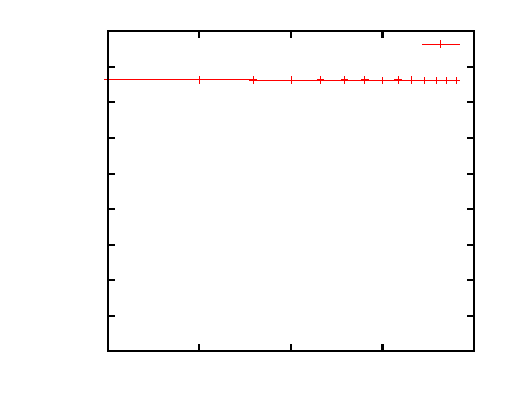
\includegraphics{CumulativeSumBlockSizeWallTimeBuild}}%
    \gplfronttext
  \end{picture}%
\endgroup

	\caption{Wall Time}
	\label{fig:CumulativeSumBuildWalltime}
\end{subfigure}
\hfill
\begin{subfigure}{0.48\textwidth}
	% GNUPLOT: LaTeX picture with Postscript
\begingroup
  \makeatletter
  \providecommand\color[2][]{%
    \GenericError{(gnuplot) \space\space\space\@spaces}{%
      Package color not loaded in conjunction with
      terminal option `colourtext'%
    }{See the gnuplot documentation for explanation.%
    }{Either use 'blacktext' in gnuplot or load the package
      color.sty in LaTeX.}%
    \renewcommand\color[2][]{}%
  }%
  \providecommand\includegraphics[2][]{%
    \GenericError{(gnuplot) \space\space\space\@spaces}{%
      Package graphicx or graphics not loaded%
    }{See the gnuplot documentation for explanation.%
    }{The gnuplot epslatex terminal needs graphicx.sty or graphics.sty.}%
    \renewcommand\includegraphics[2][]{}%
  }%
  \providecommand\rotatebox[2]{#2}%
  \@ifundefined{ifGPcolor}{%
    \newif\ifGPcolor
    \GPcolortrue
  }{}%
  \@ifundefined{ifGPblacktext}{%
    \newif\ifGPblacktext
    \GPblacktexttrue
  }{}%
  % define a \g@addto@macro without @ in the name:
  \let\gplgaddtomacro\g@addto@macro
  % define empty templates for all commands taking text:
  \gdef\gplbacktext{}%
  \gdef\gplfronttext{}%
  \makeatother
  \ifGPblacktext
    % no textcolor at all
    \def\colorrgb#1{}%
    \def\colorgray#1{}%
  \else
    % gray or color?
    \ifGPcolor
      \def\colorrgb#1{\color[rgb]{#1}}%
      \def\colorgray#1{\color[gray]{#1}}%
      \expandafter\def\csname LTw\endcsname{\color{white}}%
      \expandafter\def\csname LTb\endcsname{\color{black}}%
      \expandafter\def\csname LTa\endcsname{\color{black}}%
      \expandafter\def\csname LT0\endcsname{\color[rgb]{1,0,0}}%
      \expandafter\def\csname LT1\endcsname{\color[rgb]{0,1,0}}%
      \expandafter\def\csname LT2\endcsname{\color[rgb]{0,0,1}}%
      \expandafter\def\csname LT3\endcsname{\color[rgb]{1,0,1}}%
      \expandafter\def\csname LT4\endcsname{\color[rgb]{0,1,1}}%
      \expandafter\def\csname LT5\endcsname{\color[rgb]{1,1,0}}%
      \expandafter\def\csname LT6\endcsname{\color[rgb]{0,0,0}}%
      \expandafter\def\csname LT7\endcsname{\color[rgb]{1,0.3,0}}%
      \expandafter\def\csname LT8\endcsname{\color[rgb]{0.5,0.5,0.5}}%
    \else
      % gray
      \def\colorrgb#1{\color{black}}%
      \def\colorgray#1{\color[gray]{#1}}%
      \expandafter\def\csname LTw\endcsname{\color{white}}%
      \expandafter\def\csname LTb\endcsname{\color{black}}%
      \expandafter\def\csname LTa\endcsname{\color{black}}%
      \expandafter\def\csname LT0\endcsname{\color{black}}%
      \expandafter\def\csname LT1\endcsname{\color{black}}%
      \expandafter\def\csname LT2\endcsname{\color{black}}%
      \expandafter\def\csname LT3\endcsname{\color{black}}%
      \expandafter\def\csname LT4\endcsname{\color{black}}%
      \expandafter\def\csname LT5\endcsname{\color{black}}%
      \expandafter\def\csname LT6\endcsname{\color{black}}%
      \expandafter\def\csname LT7\endcsname{\color{black}}%
      \expandafter\def\csname LT8\endcsname{\color{black}}%
    \fi
  \fi
  \setlength{\unitlength}{0.0500bp}%
  \begin{picture}(4608.00,3600.00)%
    \gplgaddtomacro\gplbacktext{%
      \csname LTb\endcsname%
      \put(588,384){\makebox(0,0)[r]{\strut{} 700}}%
      \put(588,768){\makebox(0,0)[r]{\strut{} 800}}%
      \put(588,1152){\makebox(0,0)[r]{\strut{} 900}}%
      \put(588,1536){\makebox(0,0)[r]{\strut{} 1000}}%
      \put(588,1920){\makebox(0,0)[r]{\strut{} 1100}}%
      \put(588,2303){\makebox(0,0)[r]{\strut{} 1200}}%
      \put(588,2687){\makebox(0,0)[r]{\strut{} 1300}}%
      \put(588,3071){\makebox(0,0)[r]{\strut{} 1400}}%
      \put(588,3455){\makebox(0,0)[r]{\strut{} 1500}}%
      \put(660,264){\makebox(0,0){\strut{}$2^{2}$}}%
      \put(1193,264){\makebox(0,0){\strut{}$2^{4}$}}%
      \put(1726,264){\makebox(0,0){\strut{}$2^{6}$}}%
      \put(2259,264){\makebox(0,0){\strut{}$2^{8}$}}%
      \put(2792,264){\makebox(0,0){\strut{}$2^{10}$}}%
      \put(3325,264){\makebox(0,0){\strut{}$2^{12}$}}%
      \put(3858,264){\makebox(0,0){\strut{}$2^{14}$}}%
      \put(4391,264){\makebox(0,0){\strut{}$2^{16}$}}%
      \put(96,1919){\rotatebox{-270}{\makebox(0,0){\strut{}Memory usage (MB)}}}%
      \put(2525,84){\makebox(0,0){\strut{}Blocksize (bits)}}%
    }%
    \gplgaddtomacro\gplfronttext{%
      \csname LTb\endcsname%
      \put(3824,3332){\makebox(0,0)[r]{\strut{}CumulativeSum}}%
      \csname LTb\endcsname%
      \put(3824,3212){\makebox(0,0)[r]{\strut{}UnalignedNaive}}%
    }%
    \gplbacktext
    \put(0,0){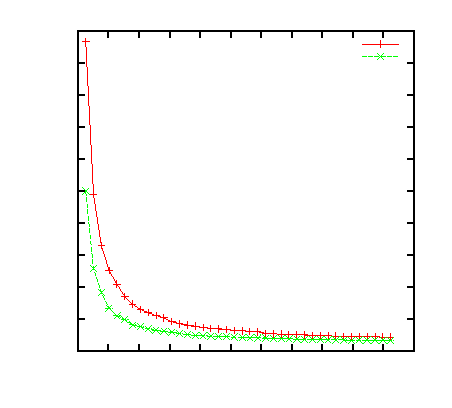
\includegraphics{CumulativeSumVsUnalignedNaiveBlockSizeBuildMemory}}%
    \gplfronttext
  \end{picture}%
\endgroup

	\caption{Memory Usage}
	\label{fig:CumulativeSumBuildMemoryUsage}
\end{subfigure}
\caption{Measurements on Building the UnalignedNaive and CumulativeSum wavelet trees. Notice that the y-axis does not start at 0.}
\label{fig:CumulativeSumBuild}
\vspace{5mm}
\begin{subfigure}{0.48\textwidth}
	% GNUPLOT: LaTeX picture with Postscript
\begingroup
  \makeatletter
  \providecommand\color[2][]{%
    \GenericError{(gnuplot) \space\space\space\@spaces}{%
      Package color not loaded in conjunction with
      terminal option `colourtext'%
    }{See the gnuplot documentation for explanation.%
    }{Either use 'blacktext' in gnuplot or load the package
      color.sty in LaTeX.}%
    \renewcommand\color[2][]{}%
  }%
  \providecommand\includegraphics[2][]{%
    \GenericError{(gnuplot) \space\space\space\@spaces}{%
      Package graphicx or graphics not loaded%
    }{See the gnuplot documentation for explanation.%
    }{The gnuplot epslatex terminal needs graphicx.sty or graphics.sty.}%
    \renewcommand\includegraphics[2][]{}%
  }%
  \providecommand\rotatebox[2]{#2}%
  \@ifundefined{ifGPcolor}{%
    \newif\ifGPcolor
    \GPcolortrue
  }{}%
  \@ifundefined{ifGPblacktext}{%
    \newif\ifGPblacktext
    \GPblacktexttrue
  }{}%
  % define a \g@addto@macro without @ in the name:
  \let\gplgaddtomacro\g@addto@macro
  % define empty templates for all commands taking text:
  \gdef\gplbacktext{}%
  \gdef\gplfronttext{}%
  \makeatother
  \ifGPblacktext
    % no textcolor at all
    \def\colorrgb#1{}%
    \def\colorgray#1{}%
  \else
    % gray or color?
    \ifGPcolor
      \def\colorrgb#1{\color[rgb]{#1}}%
      \def\colorgray#1{\color[gray]{#1}}%
      \expandafter\def\csname LTw\endcsname{\color{white}}%
      \expandafter\def\csname LTb\endcsname{\color{black}}%
      \expandafter\def\csname LTa\endcsname{\color{black}}%
      \expandafter\def\csname LT0\endcsname{\color[rgb]{1,0,0}}%
      \expandafter\def\csname LT1\endcsname{\color[rgb]{0,1,0}}%
      \expandafter\def\csname LT2\endcsname{\color[rgb]{0,0,1}}%
      \expandafter\def\csname LT3\endcsname{\color[rgb]{1,0,1}}%
      \expandafter\def\csname LT4\endcsname{\color[rgb]{0,1,1}}%
      \expandafter\def\csname LT5\endcsname{\color[rgb]{1,1,0}}%
      \expandafter\def\csname LT6\endcsname{\color[rgb]{0,0,0}}%
      \expandafter\def\csname LT7\endcsname{\color[rgb]{1,0.3,0}}%
      \expandafter\def\csname LT8\endcsname{\color[rgb]{0.5,0.5,0.5}}%
    \else
      % gray
      \def\colorrgb#1{\color{black}}%
      \def\colorgray#1{\color[gray]{#1}}%
      \expandafter\def\csname LTw\endcsname{\color{white}}%
      \expandafter\def\csname LTb\endcsname{\color{black}}%
      \expandafter\def\csname LTa\endcsname{\color{black}}%
      \expandafter\def\csname LT0\endcsname{\color{black}}%
      \expandafter\def\csname LT1\endcsname{\color{black}}%
      \expandafter\def\csname LT2\endcsname{\color{black}}%
      \expandafter\def\csname LT3\endcsname{\color{black}}%
      \expandafter\def\csname LT4\endcsname{\color{black}}%
      \expandafter\def\csname LT5\endcsname{\color{black}}%
      \expandafter\def\csname LT6\endcsname{\color{black}}%
      \expandafter\def\csname LT7\endcsname{\color{black}}%
      \expandafter\def\csname LT8\endcsname{\color{black}}%
    \fi
  \fi
  \setlength{\unitlength}{0.0500bp}%
  \begin{picture}(4608.00,3600.00)%
    \gplgaddtomacro\gplbacktext{%
      \csname LTb\endcsname%
      \put(588,384){\makebox(0,0)[r]{\strut{} 1500}}%
      \put(588,691){\makebox(0,0)[r]{\strut{} 1600}}%
      \put(588,998){\makebox(0,0)[r]{\strut{} 1700}}%
      \put(588,1305){\makebox(0,0)[r]{\strut{} 1800}}%
      \put(588,1612){\makebox(0,0)[r]{\strut{} 1900}}%
      \put(588,1920){\makebox(0,0)[r]{\strut{} 2000}}%
      \put(588,2227){\makebox(0,0)[r]{\strut{} 2100}}%
      \put(588,2534){\makebox(0,0)[r]{\strut{} 2200}}%
      \put(588,2841){\makebox(0,0)[r]{\strut{} 2300}}%
      \put(588,3148){\makebox(0,0)[r]{\strut{} 2400}}%
      \put(588,3455){\makebox(0,0)[r]{\strut{} 2500}}%
      \put(660,264){\makebox(0,0){\strut{} 0}}%
      \put(1033,264){\makebox(0,0){\strut{} 10}}%
      \put(1406,264){\makebox(0,0){\strut{} 20}}%
      \put(1779,264){\makebox(0,0){\strut{} 30}}%
      \put(2152,264){\makebox(0,0){\strut{} 40}}%
      \put(2526,264){\makebox(0,0){\strut{} 50}}%
      \put(2899,264){\makebox(0,0){\strut{} 60}}%
      \put(3272,264){\makebox(0,0){\strut{} 70}}%
      \put(3645,264){\makebox(0,0){\strut{} 80}}%
      \put(4018,264){\makebox(0,0){\strut{} 90}}%
      \put(4391,264){\makebox(0,0){\strut{} 100}}%
      \put(96,1919){\rotatebox{-270}{\makebox(0,0){\strut{}Walltime}}}%
      \put(2525,84){\makebox(0,0){\strut{}Block size (bits)}}%
    }%
    \gplgaddtomacro\gplfronttext{%
      \csname LTb\endcsname%
      \put(3824,3332){\makebox(0,0)[r]{\strut{}Rank}}%
    }%
    \gplbacktext
    \put(0,0){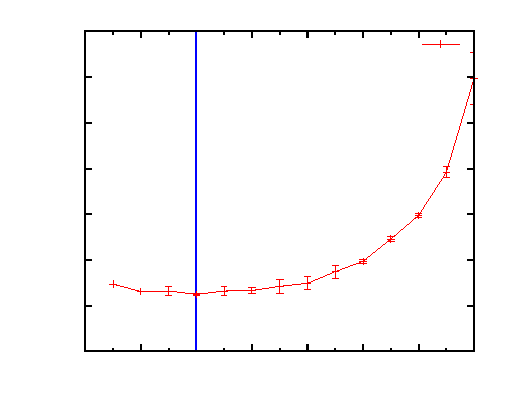
\includegraphics{CumulativeSumBlockSizeWallTimeRank}}%
    \gplfronttext
  \end{picture}%
\endgroup

	\caption{Rank. Blue line marks expected best block size.}
	\label{fig:CumulativeSumBlockSizeWallTimeRank}
\end{subfigure}
\hfill
\begin{subfigure}{0.48\textwidth}
	% GNUPLOT: LaTeX picture with Postscript
\begingroup
  \makeatletter
  \providecommand\color[2][]{%
    \GenericError{(gnuplot) \space\space\space\@spaces}{%
      Package color not loaded in conjunction with
      terminal option `colourtext'%
    }{See the gnuplot documentation for explanation.%
    }{Either use 'blacktext' in gnuplot or load the package
      color.sty in LaTeX.}%
    \renewcommand\color[2][]{}%
  }%
  \providecommand\includegraphics[2][]{%
    \GenericError{(gnuplot) \space\space\space\@spaces}{%
      Package graphicx or graphics not loaded%
    }{See the gnuplot documentation for explanation.%
    }{The gnuplot epslatex terminal needs graphicx.sty or graphics.sty.}%
    \renewcommand\includegraphics[2][]{}%
  }%
  \providecommand\rotatebox[2]{#2}%
  \@ifundefined{ifGPcolor}{%
    \newif\ifGPcolor
    \GPcolortrue
  }{}%
  \@ifundefined{ifGPblacktext}{%
    \newif\ifGPblacktext
    \GPblacktexttrue
  }{}%
  % define a \g@addto@macro without @ in the name:
  \let\gplgaddtomacro\g@addto@macro
  % define empty templates for all commands taking text:
  \gdef\gplbacktext{}%
  \gdef\gplfronttext{}%
  \makeatother
  \ifGPblacktext
    % no textcolor at all
    \def\colorrgb#1{}%
    \def\colorgray#1{}%
  \else
    % gray or color?
    \ifGPcolor
      \def\colorrgb#1{\color[rgb]{#1}}%
      \def\colorgray#1{\color[gray]{#1}}%
      \expandafter\def\csname LTw\endcsname{\color{white}}%
      \expandafter\def\csname LTb\endcsname{\color{black}}%
      \expandafter\def\csname LTa\endcsname{\color{black}}%
      \expandafter\def\csname LT0\endcsname{\color[rgb]{1,0,0}}%
      \expandafter\def\csname LT1\endcsname{\color[rgb]{0,1,0}}%
      \expandafter\def\csname LT2\endcsname{\color[rgb]{0,0,1}}%
      \expandafter\def\csname LT3\endcsname{\color[rgb]{1,0,1}}%
      \expandafter\def\csname LT4\endcsname{\color[rgb]{0,1,1}}%
      \expandafter\def\csname LT5\endcsname{\color[rgb]{1,1,0}}%
      \expandafter\def\csname LT6\endcsname{\color[rgb]{0,0,0}}%
      \expandafter\def\csname LT7\endcsname{\color[rgb]{1,0.3,0}}%
      \expandafter\def\csname LT8\endcsname{\color[rgb]{0.5,0.5,0.5}}%
    \else
      % gray
      \def\colorrgb#1{\color{black}}%
      \def\colorgray#1{\color[gray]{#1}}%
      \expandafter\def\csname LTw\endcsname{\color{white}}%
      \expandafter\def\csname LTb\endcsname{\color{black}}%
      \expandafter\def\csname LTa\endcsname{\color{black}}%
      \expandafter\def\csname LT0\endcsname{\color{black}}%
      \expandafter\def\csname LT1\endcsname{\color{black}}%
      \expandafter\def\csname LT2\endcsname{\color{black}}%
      \expandafter\def\csname LT3\endcsname{\color{black}}%
      \expandafter\def\csname LT4\endcsname{\color{black}}%
      \expandafter\def\csname LT5\endcsname{\color{black}}%
      \expandafter\def\csname LT6\endcsname{\color{black}}%
      \expandafter\def\csname LT7\endcsname{\color{black}}%
      \expandafter\def\csname LT8\endcsname{\color{black}}%
    \fi
  \fi
  \setlength{\unitlength}{0.0500bp}%
  \begin{picture}(4608.00,3600.00)%
    \gplgaddtomacro\gplbacktext{%
      \csname LTb\endcsname%
      \put(588,384){\makebox(0,0)[r]{\strut{} 6800}}%
      \put(588,896){\makebox(0,0)[r]{\strut{} 7000}}%
      \put(588,1408){\makebox(0,0)[r]{\strut{} 7200}}%
      \put(588,1920){\makebox(0,0)[r]{\strut{} 7400}}%
      \put(588,2431){\makebox(0,0)[r]{\strut{} 7600}}%
      \put(588,2943){\makebox(0,0)[r]{\strut{} 7800}}%
      \put(588,3455){\makebox(0,0)[r]{\strut{} 8000}}%
      \put(660,264){\makebox(0,0){\strut{} 0}}%
      \put(999,264){\makebox(0,0){\strut{} 500}}%
      \put(1338,264){\makebox(0,0){\strut{} 1000}}%
      \put(1678,264){\makebox(0,0){\strut{} 1500}}%
      \put(2017,264){\makebox(0,0){\strut{} 2000}}%
      \put(2356,264){\makebox(0,0){\strut{} 2500}}%
      \put(2695,264){\makebox(0,0){\strut{} 3000}}%
      \put(3034,264){\makebox(0,0){\strut{} 3500}}%
      \put(3373,264){\makebox(0,0){\strut{} 4000}}%
      \put(3713,264){\makebox(0,0){\strut{} 4500}}%
      \put(4052,264){\makebox(0,0){\strut{} 5000}}%
      \put(4391,264){\makebox(0,0){\strut{} 5500}}%
      \put(96,1919){\rotatebox{-270}{\makebox(0,0){\strut{}Walltime}}}%
      \put(2525,84){\makebox(0,0){\strut{}Blocksize (bit)}}%
    }%
    \gplgaddtomacro\gplfronttext{%
      \csname LTb\endcsname%
      \put(3824,3332){\makebox(0,0)[r]{\strut{}Select}}%
    }%
    \gplbacktext
    \put(0,0){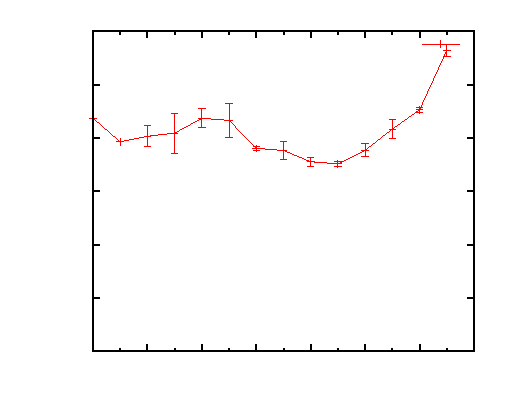
\includegraphics{CumulativeSumBlockSizeWallTimeSelect}}%
    \gplfronttext
  \end{picture}%
\endgroup

	\caption{Select.}
	\label{fig:CumulativeSumBlockSizeWallTimeSelect}
\end{subfigure}

\begin{subfigure}{0.48\textwidth}
	% GNUPLOT: LaTeX picture with Postscript
\begingroup
  \makeatletter
  \providecommand\color[2][]{%
    \GenericError{(gnuplot) \space\space\space\@spaces}{%
      Package color not loaded in conjunction with
      terminal option `colourtext'%
    }{See the gnuplot documentation for explanation.%
    }{Either use 'blacktext' in gnuplot or load the package
      color.sty in LaTeX.}%
    \renewcommand\color[2][]{}%
  }%
  \providecommand\includegraphics[2][]{%
    \GenericError{(gnuplot) \space\space\space\@spaces}{%
      Package graphicx or graphics not loaded%
    }{See the gnuplot documentation for explanation.%
    }{The gnuplot epslatex terminal needs graphicx.sty or graphics.sty.}%
    \renewcommand\includegraphics[2][]{}%
  }%
  \providecommand\rotatebox[2]{#2}%
  \@ifundefined{ifGPcolor}{%
    \newif\ifGPcolor
    \GPcolortrue
  }{}%
  \@ifundefined{ifGPblacktext}{%
    \newif\ifGPblacktext
    \GPblacktexttrue
  }{}%
  % define a \g@addto@macro without @ in the name:
  \let\gplgaddtomacro\g@addto@macro
  % define empty templates for all commands taking text:
  \gdef\gplbacktext{}%
  \gdef\gplfronttext{}%
  \makeatother
  \ifGPblacktext
    % no textcolor at all
    \def\colorrgb#1{}%
    \def\colorgray#1{}%
  \else
    % gray or color?
    \ifGPcolor
      \def\colorrgb#1{\color[rgb]{#1}}%
      \def\colorgray#1{\color[gray]{#1}}%
      \expandafter\def\csname LTw\endcsname{\color{white}}%
      \expandafter\def\csname LTb\endcsname{\color{black}}%
      \expandafter\def\csname LTa\endcsname{\color{black}}%
      \expandafter\def\csname LT0\endcsname{\color[rgb]{1,0,0}}%
      \expandafter\def\csname LT1\endcsname{\color[rgb]{0,1,0}}%
      \expandafter\def\csname LT2\endcsname{\color[rgb]{0,0,1}}%
      \expandafter\def\csname LT3\endcsname{\color[rgb]{1,0,1}}%
      \expandafter\def\csname LT4\endcsname{\color[rgb]{0,1,1}}%
      \expandafter\def\csname LT5\endcsname{\color[rgb]{1,1,0}}%
      \expandafter\def\csname LT6\endcsname{\color[rgb]{0,0,0}}%
      \expandafter\def\csname LT7\endcsname{\color[rgb]{1,0.3,0}}%
      \expandafter\def\csname LT8\endcsname{\color[rgb]{0.5,0.5,0.5}}%
    \else
      % gray
      \def\colorrgb#1{\color{black}}%
      \def\colorgray#1{\color[gray]{#1}}%
      \expandafter\def\csname LTw\endcsname{\color{white}}%
      \expandafter\def\csname LTb\endcsname{\color{black}}%
      \expandafter\def\csname LTa\endcsname{\color{black}}%
      \expandafter\def\csname LT0\endcsname{\color{black}}%
      \expandafter\def\csname LT1\endcsname{\color{black}}%
      \expandafter\def\csname LT2\endcsname{\color{black}}%
      \expandafter\def\csname LT3\endcsname{\color{black}}%
      \expandafter\def\csname LT4\endcsname{\color{black}}%
      \expandafter\def\csname LT5\endcsname{\color{black}}%
      \expandafter\def\csname LT6\endcsname{\color{black}}%
      \expandafter\def\csname LT7\endcsname{\color{black}}%
      \expandafter\def\csname LT8\endcsname{\color{black}}%
    \fi
  \fi
  \setlength{\unitlength}{0.0500bp}%
  \begin{picture}(4608.00,3600.00)%
    \gplgaddtomacro\gplbacktext{%
      \csname LTb\endcsname%
      \put(660,384){\makebox(0,0)[r]{\strut{} 0}}%
      \put(660,896){\makebox(0,0)[r]{\strut{} 2000}}%
      \put(660,1408){\makebox(0,0)[r]{\strut{} 4000}}%
      \put(660,1920){\makebox(0,0)[r]{\strut{} 6000}}%
      \put(660,2431){\makebox(0,0)[r]{\strut{} 8000}}%
      \put(660,2943){\makebox(0,0)[r]{\strut{} 10000}}%
      \put(660,3455){\makebox(0,0)[r]{\strut{} 12000}}%
      \put(732,264){\makebox(0,0){\strut{} 128}}%
      \put(1342,264){\makebox(0,0){\strut{} 256}}%
      \put(1952,264){\makebox(0,0){\strut{} 512}}%
      \put(2562,264){\makebox(0,0){\strut{} 1024}}%
      \put(3171,264){\makebox(0,0){\strut{} 2048}}%
      \put(3781,264){\makebox(0,0){\strut{} 4096}}%
      \put(4391,264){\makebox(0,0){\strut{} 8192}}%
      \put(96,1919){\rotatebox{-270}{\makebox(0,0){\strut{}Walltime}}}%
      \put(2561,84){\makebox(0,0){\strut{}Block size (bits)}}%
    }%
    \gplgaddtomacro\gplfronttext{%
      \csname LTb\endcsname%
      \put(3824,3332){\makebox(0,0)[r]{\strut{}Select, Branchless}}%
    }%
    \gplbacktext
    \put(0,0){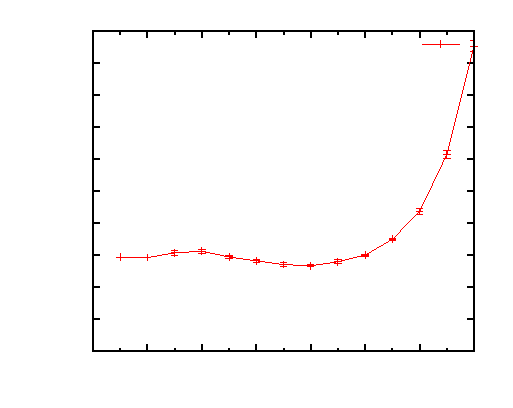
\includegraphics{CumulativeSumBlockSizeWallTimeSelectBranchless}}%
    \gplfronttext
  \end{picture}%
\endgroup

	\caption{Branchless Select.}
	\label{fig:CumulativeSumBlockSizeWallTimeSelectBranchless}
\end{subfigure}

\caption{Running times of CumulativeSum rank and select for varying block sizes with $n=10^8$ characters. Notice the x-axis (block size) is logarithmic.}
\label{fig:CumulativeSumBlockSize}
\end{figure}

\restoregeometry

\subsubsection{Rank Queries}
In Figure~\ref{fig:CumulativeSumRank} we have plotted various measurements for Rank queries on the UnalignedNaive and CumulativeSum trees.
In Figure~\ref{fig:CumulativeSumRankWalltime} we can see that storing and using the cumulative sum of rank values instead of the rank values for each block improves the running time of rank queries.
UnalignedNaive spends 3.57 milliseconds on 1000 queries, where CumulativeSum spends 3.04 milliseconds, an improvement of 14.77\,\%.

Looking at Figure~\ref{fig:CumulativeSumRankBranchMiss}, Figure~\ref{fig:CumulativeSumRankBranchMissRate}, and Figure~\ref{fig:CumulativeSumRankBranchExe} we can see that the tree using cumulative sums has much fewer branch mispredictions and a lower misprediction rate, as well as executing fewer conditional branches overall during rank queries.
This can be explained by the removal of a for-loop in CumulativeSum that iterated over the precomputed values, summing them up to calculate the rank, instead replacing it with a single lookup of a precomputed value.

In Figure~\ref{fig:CumulativeSumRankTLBMiss} we see that the CumulativeSum tree has slightly fewer Translation Lookaside Buffer Misses, although we can see from the errorbars that they their standard deviations overlap, so perhaps there is less of an improvement here than it might look like at first glance, if any at all.

In Figure~\ref{fig:CumulativeSumRankL1CM}, Figure~\ref{fig:CumulativeSumRankL2CM}, and Figure~\ref{fig:CumulativeSumRankL3CM} we can see that rank queries on the CumulativeSum wavelet tree has a much better level 1 cache performance, and only slightly worse level 2 and 3 cache performance.

In Figure~\ref{fig:CumulativeSumRankL2CHits} we can see that the amount of level 2 cache hits decrease significantly when using cumulative sums of the precomputed values.
The explanation for the decrease in level 2 cache hits might lie in the reduction of level 1 cache misses (Figure~\ref{fig:CumulativeSumRankL1CM}), like results from previous experiments.
The reduction in level 2 cache hits is simply the amount of cache lookups that the level 1 cache instead was able to handle.
The reduction of level 1 cache misses is on average $\num{135394.4}$ and the reduction in level 2 cache hits is on average $\num{133885.2}$ making them near-identical.
The level 2 cache miss rate (not shown) is therefore somewhat misleading as it would suggest a worse cache performance where the truth is that CumulativeSum has a much better cache performance, having much fewer level 1 cache misses, which helps to explain why the rank queries are faster.



\subsubsection{Select Queries}
\label{sec:cumulativeSumExperimentSelectQueries}
In Figure~\ref{fig:CumulativeSumSelect} we have plotted the same measurements as in Figure~\ref{fig:CumulativeSumRank}, but for Select queries, including our “branchless” variant of the cumulativeSum select query.

In Figure~\ref{fig:CumulativeSumSelectWalltime} we can see that storing and using the cumulative sum of precomputed rank values is also an improvement for select queries, with a reduction in wall time of 22.07\,\%.
Our “branchless” approach is also faster than not using the cumulative sum, but much slower than the simpler approach.

Looking at Figure!\ref{fig:CumulativeSumSelectBranchExe} we can see that both approaches using the cumulative sum executes much fewer conditional branches, which could be caused by using the binary search instead of having to iterate through every precomputed value from the beginning of the bitmap to the position where the sought-after occurrence lies.
Ironically, the “branchless” approach executes more conditional branches than the simple approach, which could be because it can not terminate the binary search early, resulting in execution of more branching code in the extra jumps in the binary search.

In Figure~\ref{fig:CumulativeSumSelectBranchMiss} and Figure!\ref{fig:CumulativeSumSelectBranchMissRate} we can see that the simple approach using cumulative sum has, as expected, more branch mispredictions and a higher branch misprediction rate than both the others.
The additional number of branch mispredictions contribute about $\num{508704}$ extra clock cycles, assuming 15 clock cycles per misprediction, which is only 1.87\,\% of the total number of clock cycles used in the simple approach using cumulative sum.

In Figure~\ref{fig:CumulativeSumRankTLBMiss} we can see that the simple approach also has more TLB misses than the others, yet this still has not made it slower than the others.

In Figure~\ref{fig:CumulativeSumSelectL1CM}, Figure~\ref{fig:CumulativeSumSelectL2CM}, and Figure~\ref{fig:CumulativeSumSelectL3CM} we can see that the fastest algorithm, the simple approach using cumulative sum, again has a better level 1 cache performance and worse level 2 and 3 cache performances.
The “branchless” approach has the worst level 1 cache performance and level 2 and 3 cache performances similar to the algorithm not using cumulative sum.
Again we see a reduction in level 2 cache hits in Figure~\ref{fig:CumulativeSumSelectL2CHits} from not using cumulative sum to using it, that can be, at least partially, explained by the reduction in level 1 cache misses as seen in Figure~\ref{fig:CumulativeSumSelectL1CM}.
The other part is then the increase in level 2 cache misses.

In the end we can confirm based on our measurements that it makes sense why Rank and Select is faster for CumulativeSum than for UnalignedNaive.








\newgeometry{left=2cm,right=2cm, top=2cm, bottom=3cm}
\begin{figure}\tiny

\begin{subfigure}{0.30\textwidth}
	% GNUPLOT: LaTeX picture with Postscript
\begingroup
  \makeatletter
  \providecommand\color[2][]{%
    \GenericError{(gnuplot) \space\space\space\@spaces}{%
      Package color not loaded in conjunction with
      terminal option `colourtext'%
    }{See the gnuplot documentation for explanation.%
    }{Either use 'blacktext' in gnuplot or load the package
      color.sty in LaTeX.}%
    \renewcommand\color[2][]{}%
  }%
  \providecommand\includegraphics[2][]{%
    \GenericError{(gnuplot) \space\space\space\@spaces}{%
      Package graphicx or graphics not loaded%
    }{See the gnuplot documentation for explanation.%
    }{The gnuplot epslatex terminal needs graphicx.sty or graphics.sty.}%
    \renewcommand\includegraphics[2][]{}%
  }%
  \providecommand\rotatebox[2]{#2}%
  \@ifundefined{ifGPcolor}{%
    \newif\ifGPcolor
    \GPcolortrue
  }{}%
  \@ifundefined{ifGPblacktext}{%
    \newif\ifGPblacktext
    \GPblacktexttrue
  }{}%
  % define a \g@addto@macro without @ in the name:
  \let\gplgaddtomacro\g@addto@macro
  % define empty templates for all commands taking text:
  \gdef\gplbacktext{}%
  \gdef\gplfronttext{}%
  \makeatother
  \ifGPblacktext
    % no textcolor at all
    \def\colorrgb#1{}%
    \def\colorgray#1{}%
  \else
    % gray or color?
    \ifGPcolor
      \def\colorrgb#1{\color[rgb]{#1}}%
      \def\colorgray#1{\color[gray]{#1}}%
      \expandafter\def\csname LTw\endcsname{\color{white}}%
      \expandafter\def\csname LTb\endcsname{\color{black}}%
      \expandafter\def\csname LTa\endcsname{\color{black}}%
      \expandafter\def\csname LT0\endcsname{\color[rgb]{1,0,0}}%
      \expandafter\def\csname LT1\endcsname{\color[rgb]{0,1,0}}%
      \expandafter\def\csname LT2\endcsname{\color[rgb]{0,0,1}}%
      \expandafter\def\csname LT3\endcsname{\color[rgb]{1,0,1}}%
      \expandafter\def\csname LT4\endcsname{\color[rgb]{0,1,1}}%
      \expandafter\def\csname LT5\endcsname{\color[rgb]{1,1,0}}%
      \expandafter\def\csname LT6\endcsname{\color[rgb]{0,0,0}}%
      \expandafter\def\csname LT7\endcsname{\color[rgb]{1,0.3,0}}%
      \expandafter\def\csname LT8\endcsname{\color[rgb]{0.5,0.5,0.5}}%
    \else
      % gray
      \def\colorrgb#1{\color{black}}%
      \def\colorgray#1{\color[gray]{#1}}%
      \expandafter\def\csname LTw\endcsname{\color{white}}%
      \expandafter\def\csname LTb\endcsname{\color{black}}%
      \expandafter\def\csname LTa\endcsname{\color{black}}%
      \expandafter\def\csname LT0\endcsname{\color{black}}%
      \expandafter\def\csname LT1\endcsname{\color{black}}%
      \expandafter\def\csname LT2\endcsname{\color{black}}%
      \expandafter\def\csname LT3\endcsname{\color{black}}%
      \expandafter\def\csname LT4\endcsname{\color{black}}%
      \expandafter\def\csname LT5\endcsname{\color{black}}%
      \expandafter\def\csname LT6\endcsname{\color{black}}%
      \expandafter\def\csname LT7\endcsname{\color{black}}%
      \expandafter\def\csname LT8\endcsname{\color{black}}%
    \fi
  \fi
  \setlength{\unitlength}{0.0500bp}%
  \begin{picture}(3024.00,3600.00)%
    \gplgaddtomacro\gplbacktext{%
      \csname LTb\endcsname%
      \put(559,156){\makebox(0,0)[r]{\strut{} 0}}%
      \put(559,567){\makebox(0,0)[r]{\strut{} 0.5}}%
      \put(559,978){\makebox(0,0)[r]{\strut{} 1}}%
      \put(559,1389){\makebox(0,0)[r]{\strut{} 1.5}}%
      \put(559,1800){\makebox(0,0)[r]{\strut{} 2}}%
      \put(559,2210){\makebox(0,0)[r]{\strut{} 2.5}}%
      \put(559,2621){\makebox(0,0)[r]{\strut{} 3}}%
      \put(559,3032){\makebox(0,0)[r]{\strut{} 3.5}}%
      \put(559,3443){\makebox(0,0)[r]{\strut{} 4}}%
      \put(104,1799){\rotatebox{-270}{\makebox(0,0){\strut{}Walltime (milliseconds)}}}%
    }%
    \gplgaddtomacro\gplfronttext{%
      \csname LTb\endcsname%
      \put(1807,3315){\makebox(0,0)[r]{\strut{}UnalignedNaive}}%
      \csname LTb\endcsname%
      \put(1807,3185){\makebox(0,0)[r]{\strut{}CumulativeSum}}%
    }%
    \gplbacktext
    \put(0,0){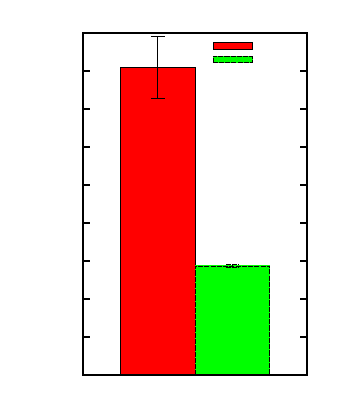
\includegraphics{CumulativeSumRankWalltime}}%
    \gplfronttext
  \end{picture}%
\endgroup

	\caption{Wall Time}
	\label{fig:CumulativeSumRankWalltime}
\end{subfigure}
\hfill
\begin{subfigure}{0.30\textwidth}
	% GNUPLOT: LaTeX picture with Postscript
\begingroup
  \makeatletter
  \providecommand\color[2][]{%
    \GenericError{(gnuplot) \space\space\space\@spaces}{%
      Package color not loaded in conjunction with
      terminal option `colourtext'%
    }{See the gnuplot documentation for explanation.%
    }{Either use 'blacktext' in gnuplot or load the package
      color.sty in LaTeX.}%
    \renewcommand\color[2][]{}%
  }%
  \providecommand\includegraphics[2][]{%
    \GenericError{(gnuplot) \space\space\space\@spaces}{%
      Package graphicx or graphics not loaded%
    }{See the gnuplot documentation for explanation.%
    }{The gnuplot epslatex terminal needs graphicx.sty or graphics.sty.}%
    \renewcommand\includegraphics[2][]{}%
  }%
  \providecommand\rotatebox[2]{#2}%
  \@ifundefined{ifGPcolor}{%
    \newif\ifGPcolor
    \GPcolortrue
  }{}%
  \@ifundefined{ifGPblacktext}{%
    \newif\ifGPblacktext
    \GPblacktexttrue
  }{}%
  % define a \g@addto@macro without @ in the name:
  \let\gplgaddtomacro\g@addto@macro
  % define empty templates for all commands taking text:
  \gdef\gplbacktext{}%
  \gdef\gplfronttext{}%
  \makeatother
  \ifGPblacktext
    % no textcolor at all
    \def\colorrgb#1{}%
    \def\colorgray#1{}%
  \else
    % gray or color?
    \ifGPcolor
      \def\colorrgb#1{\color[rgb]{#1}}%
      \def\colorgray#1{\color[gray]{#1}}%
      \expandafter\def\csname LTw\endcsname{\color{white}}%
      \expandafter\def\csname LTb\endcsname{\color{black}}%
      \expandafter\def\csname LTa\endcsname{\color{black}}%
      \expandafter\def\csname LT0\endcsname{\color[rgb]{1,0,0}}%
      \expandafter\def\csname LT1\endcsname{\color[rgb]{0,1,0}}%
      \expandafter\def\csname LT2\endcsname{\color[rgb]{0,0,1}}%
      \expandafter\def\csname LT3\endcsname{\color[rgb]{1,0,1}}%
      \expandafter\def\csname LT4\endcsname{\color[rgb]{0,1,1}}%
      \expandafter\def\csname LT5\endcsname{\color[rgb]{1,1,0}}%
      \expandafter\def\csname LT6\endcsname{\color[rgb]{0,0,0}}%
      \expandafter\def\csname LT7\endcsname{\color[rgb]{1,0.3,0}}%
      \expandafter\def\csname LT8\endcsname{\color[rgb]{0.5,0.5,0.5}}%
    \else
      % gray
      \def\colorrgb#1{\color{black}}%
      \def\colorgray#1{\color[gray]{#1}}%
      \expandafter\def\csname LTw\endcsname{\color{white}}%
      \expandafter\def\csname LTb\endcsname{\color{black}}%
      \expandafter\def\csname LTa\endcsname{\color{black}}%
      \expandafter\def\csname LT0\endcsname{\color{black}}%
      \expandafter\def\csname LT1\endcsname{\color{black}}%
      \expandafter\def\csname LT2\endcsname{\color{black}}%
      \expandafter\def\csname LT3\endcsname{\color{black}}%
      \expandafter\def\csname LT4\endcsname{\color{black}}%
      \expandafter\def\csname LT5\endcsname{\color{black}}%
      \expandafter\def\csname LT6\endcsname{\color{black}}%
      \expandafter\def\csname LT7\endcsname{\color{black}}%
      \expandafter\def\csname LT8\endcsname{\color{black}}%
    \fi
  \fi
  \setlength{\unitlength}{0.0500bp}%
  \begin{picture}(3024.00,3600.00)%
    \gplgaddtomacro\gplbacktext{%
      \csname LTb\endcsname%
      \put(715,156){\makebox(0,0)[r]{\strut{} 0}}%
      \put(715,513){\makebox(0,0)[r]{\strut{} 5000}}%
      \put(715,871){\makebox(0,0)[r]{\strut{} 10000}}%
      \put(715,1228){\makebox(0,0)[r]{\strut{} 15000}}%
      \put(715,1585){\makebox(0,0)[r]{\strut{} 20000}}%
      \put(715,1942){\makebox(0,0)[r]{\strut{} 25000}}%
      \put(715,2300){\makebox(0,0)[r]{\strut{} 30000}}%
      \put(715,2657){\makebox(0,0)[r]{\strut{} 35000}}%
      \put(715,3014){\makebox(0,0)[r]{\strut{} 40000}}%
      \put(715,3372){\makebox(0,0)[r]{\strut{} 45000}}%
      \put(104,1799){\rotatebox{-270}{\makebox(0,0){\strut{}Branch Misses}}}%
    }%
    \gplgaddtomacro\gplfronttext{%
      \csname LTb\endcsname%
      \put(1963,3315){\makebox(0,0)[r]{\strut{}UnalignedNaive}}%
      \csname LTb\endcsname%
      \put(1963,3185){\makebox(0,0)[r]{\strut{}CumulativeSum}}%
    }%
    \gplbacktext
    \put(0,0){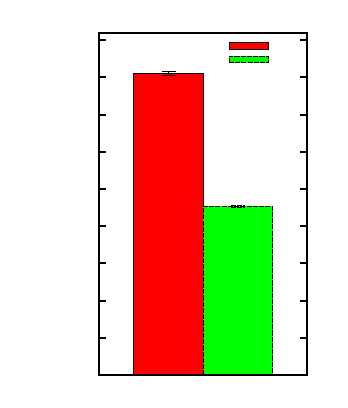
\includegraphics{CumulativeSumRankBranchMiss}}%
    \gplfronttext
  \end{picture}%
\endgroup

	\caption{Branch Mispredictions}
	\label{fig:CumulativeSumRankBranchMiss}
\end{subfigure}
\hfill
\begin{subfigure}{0.30\textwidth}
	% GNUPLOT: LaTeX picture with Postscript
\begingroup
  \makeatletter
  \providecommand\color[2][]{%
    \GenericError{(gnuplot) \space\space\space\@spaces}{%
      Package color not loaded in conjunction with
      terminal option `colourtext'%
    }{See the gnuplot documentation for explanation.%
    }{Either use 'blacktext' in gnuplot or load the package
      color.sty in LaTeX.}%
    \renewcommand\color[2][]{}%
  }%
  \providecommand\includegraphics[2][]{%
    \GenericError{(gnuplot) \space\space\space\@spaces}{%
      Package graphicx or graphics not loaded%
    }{See the gnuplot documentation for explanation.%
    }{The gnuplot epslatex terminal needs graphicx.sty or graphics.sty.}%
    \renewcommand\includegraphics[2][]{}%
  }%
  \providecommand\rotatebox[2]{#2}%
  \@ifundefined{ifGPcolor}{%
    \newif\ifGPcolor
    \GPcolortrue
  }{}%
  \@ifundefined{ifGPblacktext}{%
    \newif\ifGPblacktext
    \GPblacktexttrue
  }{}%
  % define a \g@addto@macro without @ in the name:
  \let\gplgaddtomacro\g@addto@macro
  % define empty templates for all commands taking text:
  \gdef\gplbacktext{}%
  \gdef\gplfronttext{}%
  \makeatother
  \ifGPblacktext
    % no textcolor at all
    \def\colorrgb#1{}%
    \def\colorgray#1{}%
  \else
    % gray or color?
    \ifGPcolor
      \def\colorrgb#1{\color[rgb]{#1}}%
      \def\colorgray#1{\color[gray]{#1}}%
      \expandafter\def\csname LTw\endcsname{\color{white}}%
      \expandafter\def\csname LTb\endcsname{\color{black}}%
      \expandafter\def\csname LTa\endcsname{\color{black}}%
      \expandafter\def\csname LT0\endcsname{\color[rgb]{1,0,0}}%
      \expandafter\def\csname LT1\endcsname{\color[rgb]{0,1,0}}%
      \expandafter\def\csname LT2\endcsname{\color[rgb]{0,0,1}}%
      \expandafter\def\csname LT3\endcsname{\color[rgb]{1,0,1}}%
      \expandafter\def\csname LT4\endcsname{\color[rgb]{0,1,1}}%
      \expandafter\def\csname LT5\endcsname{\color[rgb]{1,1,0}}%
      \expandafter\def\csname LT6\endcsname{\color[rgb]{0,0,0}}%
      \expandafter\def\csname LT7\endcsname{\color[rgb]{1,0.3,0}}%
      \expandafter\def\csname LT8\endcsname{\color[rgb]{0.5,0.5,0.5}}%
    \else
      % gray
      \def\colorrgb#1{\color{black}}%
      \def\colorgray#1{\color[gray]{#1}}%
      \expandafter\def\csname LTw\endcsname{\color{white}}%
      \expandafter\def\csname LTb\endcsname{\color{black}}%
      \expandafter\def\csname LTa\endcsname{\color{black}}%
      \expandafter\def\csname LT0\endcsname{\color{black}}%
      \expandafter\def\csname LT1\endcsname{\color{black}}%
      \expandafter\def\csname LT2\endcsname{\color{black}}%
      \expandafter\def\csname LT3\endcsname{\color{black}}%
      \expandafter\def\csname LT4\endcsname{\color{black}}%
      \expandafter\def\csname LT5\endcsname{\color{black}}%
      \expandafter\def\csname LT6\endcsname{\color{black}}%
      \expandafter\def\csname LT7\endcsname{\color{black}}%
      \expandafter\def\csname LT8\endcsname{\color{black}}%
    \fi
  \fi
  \setlength{\unitlength}{0.0500bp}%
  \begin{picture}(4608.00,3600.00)%
    \gplgaddtomacro\gplbacktext{%
      \csname LTb\endcsname%
      \put(871,156){\makebox(0,0)[r]{\strut{} 0}}%
      \put(871,776){\makebox(0,0)[r]{\strut{} 500000}}%
      \put(871,1396){\makebox(0,0)[r]{\strut{} 1e+06}}%
      \put(871,2017){\makebox(0,0)[r]{\strut{} 1.5e+06}}%
      \put(871,2637){\makebox(0,0)[r]{\strut{} 2e+06}}%
      \put(871,3257){\makebox(0,0)[r]{\strut{} 2.5e+06}}%
      \put(104,1799){\rotatebox{-270}{\makebox(0,0){\strut{}Branches Executed}}}%
    }%
    \gplgaddtomacro\gplfronttext{%
      \csname LTb\endcsname%
      \put(2119,3315){\makebox(0,0)[r]{\strut{}UnalignedNaive}}%
      \csname LTb\endcsname%
      \put(3742,3315){\makebox(0,0)[r]{\strut{}CumulativeSum}}%
    }%
    \gplbacktext
    \put(0,0){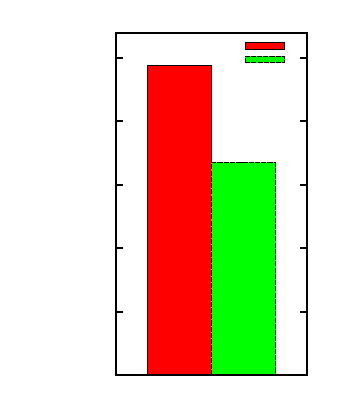
\includegraphics{CumulativeSumRankBranchExe}}%
    \gplfronttext
  \end{picture}%
\endgroup

	\caption{Branches Executed}
	\label{fig:CumulativeSumRankBranchExe}
\end{subfigure}


\begin{subfigure}{0.30\textwidth}
	% GNUPLOT: LaTeX picture with Postscript
\begingroup
  \makeatletter
  \providecommand\color[2][]{%
    \GenericError{(gnuplot) \space\space\space\@spaces}{%
      Package color not loaded in conjunction with
      terminal option `colourtext'%
    }{See the gnuplot documentation for explanation.%
    }{Either use 'blacktext' in gnuplot or load the package
      color.sty in LaTeX.}%
    \renewcommand\color[2][]{}%
  }%
  \providecommand\includegraphics[2][]{%
    \GenericError{(gnuplot) \space\space\space\@spaces}{%
      Package graphicx or graphics not loaded%
    }{See the gnuplot documentation for explanation.%
    }{The gnuplot epslatex terminal needs graphicx.sty or graphics.sty.}%
    \renewcommand\includegraphics[2][]{}%
  }%
  \providecommand\rotatebox[2]{#2}%
  \@ifundefined{ifGPcolor}{%
    \newif\ifGPcolor
    \GPcolortrue
  }{}%
  \@ifundefined{ifGPblacktext}{%
    \newif\ifGPblacktext
    \GPblacktexttrue
  }{}%
  % define a \g@addto@macro without @ in the name:
  \let\gplgaddtomacro\g@addto@macro
  % define empty templates for all commands taking text:
  \gdef\gplbacktext{}%
  \gdef\gplfronttext{}%
  \makeatother
  \ifGPblacktext
    % no textcolor at all
    \def\colorrgb#1{}%
    \def\colorgray#1{}%
  \else
    % gray or color?
    \ifGPcolor
      \def\colorrgb#1{\color[rgb]{#1}}%
      \def\colorgray#1{\color[gray]{#1}}%
      \expandafter\def\csname LTw\endcsname{\color{white}}%
      \expandafter\def\csname LTb\endcsname{\color{black}}%
      \expandafter\def\csname LTa\endcsname{\color{black}}%
      \expandafter\def\csname LT0\endcsname{\color[rgb]{1,0,0}}%
      \expandafter\def\csname LT1\endcsname{\color[rgb]{0,1,0}}%
      \expandafter\def\csname LT2\endcsname{\color[rgb]{0,0,1}}%
      \expandafter\def\csname LT3\endcsname{\color[rgb]{1,0,1}}%
      \expandafter\def\csname LT4\endcsname{\color[rgb]{0,1,1}}%
      \expandafter\def\csname LT5\endcsname{\color[rgb]{1,1,0}}%
      \expandafter\def\csname LT6\endcsname{\color[rgb]{0,0,0}}%
      \expandafter\def\csname LT7\endcsname{\color[rgb]{1,0.3,0}}%
      \expandafter\def\csname LT8\endcsname{\color[rgb]{0.5,0.5,0.5}}%
    \else
      % gray
      \def\colorrgb#1{\color{black}}%
      \def\colorgray#1{\color[gray]{#1}}%
      \expandafter\def\csname LTw\endcsname{\color{white}}%
      \expandafter\def\csname LTb\endcsname{\color{black}}%
      \expandafter\def\csname LTa\endcsname{\color{black}}%
      \expandafter\def\csname LT0\endcsname{\color{black}}%
      \expandafter\def\csname LT1\endcsname{\color{black}}%
      \expandafter\def\csname LT2\endcsname{\color{black}}%
      \expandafter\def\csname LT3\endcsname{\color{black}}%
      \expandafter\def\csname LT4\endcsname{\color{black}}%
      \expandafter\def\csname LT5\endcsname{\color{black}}%
      \expandafter\def\csname LT6\endcsname{\color{black}}%
      \expandafter\def\csname LT7\endcsname{\color{black}}%
      \expandafter\def\csname LT8\endcsname{\color{black}}%
    \fi
  \fi
  \setlength{\unitlength}{0.0500bp}%
  \begin{picture}(3024.00,3600.00)%
    \gplgaddtomacro\gplbacktext{%
      \csname LTb\endcsname%
      \put(637,156){\makebox(0,0)[r]{\strut{} 0}}%
      \put(637,662){\makebox(0,0)[r]{\strut{} 0.02}}%
      \put(637,1167){\makebox(0,0)[r]{\strut{} 0.04}}%
      \put(637,1673){\makebox(0,0)[r]{\strut{} 0.06}}%
      \put(637,2179){\makebox(0,0)[r]{\strut{} 0.08}}%
      \put(637,2684){\makebox(0,0)[r]{\strut{} 0.1}}%
      \put(637,3190){\makebox(0,0)[r]{\strut{} 0.12}}%
      \put(104,1799){\rotatebox{-270}{\makebox(0,0){\strut{}Branch Misprediction Rate}}}%
    }%
    \gplgaddtomacro\gplfronttext{%
      \csname LTb\endcsname%
      \put(1885,3315){\makebox(0,0)[r]{\strut{}UnalignedNaive}}%
      \csname LTb\endcsname%
      \put(1885,3185){\makebox(0,0)[r]{\strut{}CumulativeSum}}%
    }%
    \gplbacktext
    \put(0,0){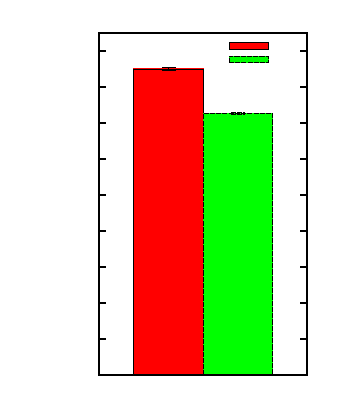
\includegraphics{CumulativeSumRankBranchMissRate}}%
    \gplfronttext
  \end{picture}%
\endgroup

	\caption{Branch Misprediction Rate}
	\label{fig:CumulativeSumRankBranchMissRate}
\end{subfigure}
\hfill
\begin{subfigure}{0.30\textwidth}
	% GNUPLOT: LaTeX picture with Postscript
\begingroup
  \makeatletter
  \providecommand\color[2][]{%
    \GenericError{(gnuplot) \space\space\space\@spaces}{%
      Package color not loaded in conjunction with
      terminal option `colourtext'%
    }{See the gnuplot documentation for explanation.%
    }{Either use 'blacktext' in gnuplot or load the package
      color.sty in LaTeX.}%
    \renewcommand\color[2][]{}%
  }%
  \providecommand\includegraphics[2][]{%
    \GenericError{(gnuplot) \space\space\space\@spaces}{%
      Package graphicx or graphics not loaded%
    }{See the gnuplot documentation for explanation.%
    }{The gnuplot epslatex terminal needs graphicx.sty or graphics.sty.}%
    \renewcommand\includegraphics[2][]{}%
  }%
  \providecommand\rotatebox[2]{#2}%
  \@ifundefined{ifGPcolor}{%
    \newif\ifGPcolor
    \GPcolortrue
  }{}%
  \@ifundefined{ifGPblacktext}{%
    \newif\ifGPblacktext
    \GPblacktexttrue
  }{}%
  % define a \g@addto@macro without @ in the name:
  \let\gplgaddtomacro\g@addto@macro
  % define empty templates for all commands taking text:
  \gdef\gplbacktext{}%
  \gdef\gplfronttext{}%
  \makeatother
  \ifGPblacktext
    % no textcolor at all
    \def\colorrgb#1{}%
    \def\colorgray#1{}%
  \else
    % gray or color?
    \ifGPcolor
      \def\colorrgb#1{\color[rgb]{#1}}%
      \def\colorgray#1{\color[gray]{#1}}%
      \expandafter\def\csname LTw\endcsname{\color{white}}%
      \expandafter\def\csname LTb\endcsname{\color{black}}%
      \expandafter\def\csname LTa\endcsname{\color{black}}%
      \expandafter\def\csname LT0\endcsname{\color[rgb]{1,0,0}}%
      \expandafter\def\csname LT1\endcsname{\color[rgb]{0,1,0}}%
      \expandafter\def\csname LT2\endcsname{\color[rgb]{0,0,1}}%
      \expandafter\def\csname LT3\endcsname{\color[rgb]{1,0,1}}%
      \expandafter\def\csname LT4\endcsname{\color[rgb]{0,1,1}}%
      \expandafter\def\csname LT5\endcsname{\color[rgb]{1,1,0}}%
      \expandafter\def\csname LT6\endcsname{\color[rgb]{0,0,0}}%
      \expandafter\def\csname LT7\endcsname{\color[rgb]{1,0.3,0}}%
      \expandafter\def\csname LT8\endcsname{\color[rgb]{0.5,0.5,0.5}}%
    \else
      % gray
      \def\colorrgb#1{\color{black}}%
      \def\colorgray#1{\color[gray]{#1}}%
      \expandafter\def\csname LTw\endcsname{\color{white}}%
      \expandafter\def\csname LTb\endcsname{\color{black}}%
      \expandafter\def\csname LTa\endcsname{\color{black}}%
      \expandafter\def\csname LT0\endcsname{\color{black}}%
      \expandafter\def\csname LT1\endcsname{\color{black}}%
      \expandafter\def\csname LT2\endcsname{\color{black}}%
      \expandafter\def\csname LT3\endcsname{\color{black}}%
      \expandafter\def\csname LT4\endcsname{\color{black}}%
      \expandafter\def\csname LT5\endcsname{\color{black}}%
      \expandafter\def\csname LT6\endcsname{\color{black}}%
      \expandafter\def\csname LT7\endcsname{\color{black}}%
      \expandafter\def\csname LT8\endcsname{\color{black}}%
    \fi
  \fi
  \setlength{\unitlength}{0.0500bp}%
  \begin{picture}(4608.00,3600.00)%
    \gplgaddtomacro\gplbacktext{%
      \csname LTb\endcsname%
      \put(637,156){\makebox(0,0)[r]{\strut{} 0}}%
      \put(637,704){\makebox(0,0)[r]{\strut{} 1000}}%
      \put(637,1252){\makebox(0,0)[r]{\strut{} 2000}}%
      \put(637,1799){\makebox(0,0)[r]{\strut{} 3000}}%
      \put(637,2347){\makebox(0,0)[r]{\strut{} 4000}}%
      \put(637,2895){\makebox(0,0)[r]{\strut{} 5000}}%
      \put(637,3443){\makebox(0,0)[r]{\strut{} 6000}}%
      \put(104,1799){\rotatebox{-270}{\makebox(0,0){\strut{}TLB Misses}}}%
    }%
    \gplgaddtomacro\gplfronttext{%
      \csname LTb\endcsname%
      \put(1885,3315){\makebox(0,0)[r]{\strut{}UnalignedNaive}}%
      \csname LTb\endcsname%
      \put(3508,3315){\makebox(0,0)[r]{\strut{}CumulativeSum}}%
    }%
    \gplbacktext
    \put(0,0){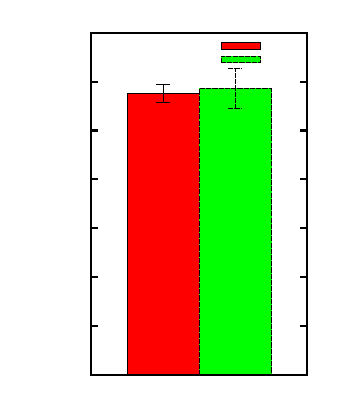
\includegraphics{CumulativeSumRankTLBMiss}}%
    \gplfronttext
  \end{picture}%
\endgroup

	\caption{TLB Misses}
	\label{fig:CumulativeSumRankTLBMiss}
\end{subfigure}
\hfill
\begin{subfigure}{0.30\textwidth}
	% GNUPLOT: LaTeX picture with Postscript
\begingroup
  \makeatletter
  \providecommand\color[2][]{%
    \GenericError{(gnuplot) \space\space\space\@spaces}{%
      Package color not loaded in conjunction with
      terminal option `colourtext'%
    }{See the gnuplot documentation for explanation.%
    }{Either use 'blacktext' in gnuplot or load the package
      color.sty in LaTeX.}%
    \renewcommand\color[2][]{}%
  }%
  \providecommand\includegraphics[2][]{%
    \GenericError{(gnuplot) \space\space\space\@spaces}{%
      Package graphicx or graphics not loaded%
    }{See the gnuplot documentation for explanation.%
    }{The gnuplot epslatex terminal needs graphicx.sty or graphics.sty.}%
    \renewcommand\includegraphics[2][]{}%
  }%
  \providecommand\rotatebox[2]{#2}%
  \@ifundefined{ifGPcolor}{%
    \newif\ifGPcolor
    \GPcolortrue
  }{}%
  \@ifundefined{ifGPblacktext}{%
    \newif\ifGPblacktext
    \GPblacktexttrue
  }{}%
  % define a \g@addto@macro without @ in the name:
  \let\gplgaddtomacro\g@addto@macro
  % define empty templates for all commands taking text:
  \gdef\gplbacktext{}%
  \gdef\gplfronttext{}%
  \makeatother
  \ifGPblacktext
    % no textcolor at all
    \def\colorrgb#1{}%
    \def\colorgray#1{}%
  \else
    % gray or color?
    \ifGPcolor
      \def\colorrgb#1{\color[rgb]{#1}}%
      \def\colorgray#1{\color[gray]{#1}}%
      \expandafter\def\csname LTw\endcsname{\color{white}}%
      \expandafter\def\csname LTb\endcsname{\color{black}}%
      \expandafter\def\csname LTa\endcsname{\color{black}}%
      \expandafter\def\csname LT0\endcsname{\color[rgb]{1,0,0}}%
      \expandafter\def\csname LT1\endcsname{\color[rgb]{0,1,0}}%
      \expandafter\def\csname LT2\endcsname{\color[rgb]{0,0,1}}%
      \expandafter\def\csname LT3\endcsname{\color[rgb]{1,0,1}}%
      \expandafter\def\csname LT4\endcsname{\color[rgb]{0,1,1}}%
      \expandafter\def\csname LT5\endcsname{\color[rgb]{1,1,0}}%
      \expandafter\def\csname LT6\endcsname{\color[rgb]{0,0,0}}%
      \expandafter\def\csname LT7\endcsname{\color[rgb]{1,0.3,0}}%
      \expandafter\def\csname LT8\endcsname{\color[rgb]{0.5,0.5,0.5}}%
    \else
      % gray
      \def\colorrgb#1{\color{black}}%
      \def\colorgray#1{\color[gray]{#1}}%
      \expandafter\def\csname LTw\endcsname{\color{white}}%
      \expandafter\def\csname LTb\endcsname{\color{black}}%
      \expandafter\def\csname LTa\endcsname{\color{black}}%
      \expandafter\def\csname LT0\endcsname{\color{black}}%
      \expandafter\def\csname LT1\endcsname{\color{black}}%
      \expandafter\def\csname LT2\endcsname{\color{black}}%
      \expandafter\def\csname LT3\endcsname{\color{black}}%
      \expandafter\def\csname LT4\endcsname{\color{black}}%
      \expandafter\def\csname LT5\endcsname{\color{black}}%
      \expandafter\def\csname LT6\endcsname{\color{black}}%
      \expandafter\def\csname LT7\endcsname{\color{black}}%
      \expandafter\def\csname LT8\endcsname{\color{black}}%
    \fi
  \fi
  \setlength{\unitlength}{0.0500bp}%
  \begin{picture}(4608.00,3600.00)%
    \gplgaddtomacro\gplbacktext{%
      \csname LTb\endcsname%
      \put(793,156){\makebox(0,0)[r]{\strut{} 0}}%
      \put(793,521){\makebox(0,0)[r]{\strut{} 50000}}%
      \put(793,886){\makebox(0,0)[r]{\strut{} 100000}}%
      \put(793,1252){\makebox(0,0)[r]{\strut{} 150000}}%
      \put(793,1617){\makebox(0,0)[r]{\strut{} 200000}}%
      \put(793,1982){\makebox(0,0)[r]{\strut{} 250000}}%
      \put(793,2347){\makebox(0,0)[r]{\strut{} 300000}}%
      \put(793,2713){\makebox(0,0)[r]{\strut{} 350000}}%
      \put(793,3078){\makebox(0,0)[r]{\strut{} 400000}}%
      \put(793,3443){\makebox(0,0)[r]{\strut{} 450000}}%
      \put(104,1799){\rotatebox{-270}{\makebox(0,0){\strut{}Cache Misses}}}%
    }%
    \gplgaddtomacro\gplfronttext{%
      \csname LTb\endcsname%
      \put(2041,3315){\makebox(0,0)[r]{\strut{}UnalignedNaive}}%
      \csname LTb\endcsname%
      \put(3664,3315){\makebox(0,0)[r]{\strut{}CumulativeSum}}%
    }%
    \gplbacktext
    \put(0,0){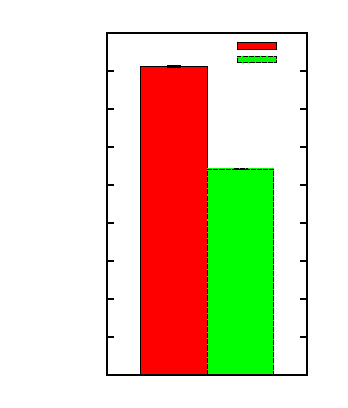
\includegraphics{CumulativeSumRankL1CM}}%
    \gplfronttext
  \end{picture}%
\endgroup

	\caption{Level 1 Cache Misses}
	\label{fig:CumulativeSumRankL1CM}
\end{subfigure}

\begin{subfigure}{0.30\textwidth}
	% GNUPLOT: LaTeX picture with Postscript
\begingroup
  \makeatletter
  \providecommand\color[2][]{%
    \GenericError{(gnuplot) \space\space\space\@spaces}{%
      Package color not loaded in conjunction with
      terminal option `colourtext'%
    }{See the gnuplot documentation for explanation.%
    }{Either use 'blacktext' in gnuplot or load the package
      color.sty in LaTeX.}%
    \renewcommand\color[2][]{}%
  }%
  \providecommand\includegraphics[2][]{%
    \GenericError{(gnuplot) \space\space\space\@spaces}{%
      Package graphicx or graphics not loaded%
    }{See the gnuplot documentation for explanation.%
    }{The gnuplot epslatex terminal needs graphicx.sty or graphics.sty.}%
    \renewcommand\includegraphics[2][]{}%
  }%
  \providecommand\rotatebox[2]{#2}%
  \@ifundefined{ifGPcolor}{%
    \newif\ifGPcolor
    \GPcolortrue
  }{}%
  \@ifundefined{ifGPblacktext}{%
    \newif\ifGPblacktext
    \GPblacktexttrue
  }{}%
  % define a \g@addto@macro without @ in the name:
  \let\gplgaddtomacro\g@addto@macro
  % define empty templates for all commands taking text:
  \gdef\gplbacktext{}%
  \gdef\gplfronttext{}%
  \makeatother
  \ifGPblacktext
    % no textcolor at all
    \def\colorrgb#1{}%
    \def\colorgray#1{}%
  \else
    % gray or color?
    \ifGPcolor
      \def\colorrgb#1{\color[rgb]{#1}}%
      \def\colorgray#1{\color[gray]{#1}}%
      \expandafter\def\csname LTw\endcsname{\color{white}}%
      \expandafter\def\csname LTb\endcsname{\color{black}}%
      \expandafter\def\csname LTa\endcsname{\color{black}}%
      \expandafter\def\csname LT0\endcsname{\color[rgb]{1,0,0}}%
      \expandafter\def\csname LT1\endcsname{\color[rgb]{0,1,0}}%
      \expandafter\def\csname LT2\endcsname{\color[rgb]{0,0,1}}%
      \expandafter\def\csname LT3\endcsname{\color[rgb]{1,0,1}}%
      \expandafter\def\csname LT4\endcsname{\color[rgb]{0,1,1}}%
      \expandafter\def\csname LT5\endcsname{\color[rgb]{1,1,0}}%
      \expandafter\def\csname LT6\endcsname{\color[rgb]{0,0,0}}%
      \expandafter\def\csname LT7\endcsname{\color[rgb]{1,0.3,0}}%
      \expandafter\def\csname LT8\endcsname{\color[rgb]{0.5,0.5,0.5}}%
    \else
      % gray
      \def\colorrgb#1{\color{black}}%
      \def\colorgray#1{\color[gray]{#1}}%
      \expandafter\def\csname LTw\endcsname{\color{white}}%
      \expandafter\def\csname LTb\endcsname{\color{black}}%
      \expandafter\def\csname LTa\endcsname{\color{black}}%
      \expandafter\def\csname LT0\endcsname{\color{black}}%
      \expandafter\def\csname LT1\endcsname{\color{black}}%
      \expandafter\def\csname LT2\endcsname{\color{black}}%
      \expandafter\def\csname LT3\endcsname{\color{black}}%
      \expandafter\def\csname LT4\endcsname{\color{black}}%
      \expandafter\def\csname LT5\endcsname{\color{black}}%
      \expandafter\def\csname LT6\endcsname{\color{black}}%
      \expandafter\def\csname LT7\endcsname{\color{black}}%
      \expandafter\def\csname LT8\endcsname{\color{black}}%
    \fi
  \fi
  \setlength{\unitlength}{0.0500bp}%
  \begin{picture}(4608.00,3600.00)%
    \gplgaddtomacro\gplbacktext{%
      \csname LTb\endcsname%
      \put(793,156){\makebox(0,0)[r]{\strut{} 0}}%
      \put(793,521){\makebox(0,0)[r]{\strut{} 20000}}%
      \put(793,886){\makebox(0,0)[r]{\strut{} 40000}}%
      \put(793,1252){\makebox(0,0)[r]{\strut{} 60000}}%
      \put(793,1617){\makebox(0,0)[r]{\strut{} 80000}}%
      \put(793,1982){\makebox(0,0)[r]{\strut{} 100000}}%
      \put(793,2347){\makebox(0,0)[r]{\strut{} 120000}}%
      \put(793,2713){\makebox(0,0)[r]{\strut{} 140000}}%
      \put(793,3078){\makebox(0,0)[r]{\strut{} 160000}}%
      \put(793,3443){\makebox(0,0)[r]{\strut{} 180000}}%
      \put(104,1799){\rotatebox{-270}{\makebox(0,0){\strut{}Cache Misses}}}%
    }%
    \gplgaddtomacro\gplfronttext{%
      \csname LTb\endcsname%
      \put(2041,3315){\makebox(0,0)[r]{\strut{}UnalignedNaive}}%
      \csname LTb\endcsname%
      \put(3664,3315){\makebox(0,0)[r]{\strut{}CumulativeSum}}%
    }%
    \gplbacktext
    \put(0,0){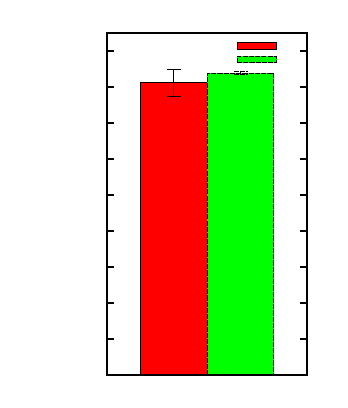
\includegraphics{CumulativeSumRankL2CM}}%
    \gplfronttext
  \end{picture}%
\endgroup

	\caption{Level 2 Cache Misses}
	\label{fig:CumulativeSumRankL2CM}
\end{subfigure}
\hfill
\begin{subfigure}{0.30\textwidth}
	% GNUPLOT: LaTeX picture with Postscript
\begingroup
  \makeatletter
  \providecommand\color[2][]{%
    \GenericError{(gnuplot) \space\space\space\@spaces}{%
      Package color not loaded in conjunction with
      terminal option `colourtext'%
    }{See the gnuplot documentation for explanation.%
    }{Either use 'blacktext' in gnuplot or load the package
      color.sty in LaTeX.}%
    \renewcommand\color[2][]{}%
  }%
  \providecommand\includegraphics[2][]{%
    \GenericError{(gnuplot) \space\space\space\@spaces}{%
      Package graphicx or graphics not loaded%
    }{See the gnuplot documentation for explanation.%
    }{The gnuplot epslatex terminal needs graphicx.sty or graphics.sty.}%
    \renewcommand\includegraphics[2][]{}%
  }%
  \providecommand\rotatebox[2]{#2}%
  \@ifundefined{ifGPcolor}{%
    \newif\ifGPcolor
    \GPcolortrue
  }{}%
  \@ifundefined{ifGPblacktext}{%
    \newif\ifGPblacktext
    \GPblacktexttrue
  }{}%
  % define a \g@addto@macro without @ in the name:
  \let\gplgaddtomacro\g@addto@macro
  % define empty templates for all commands taking text:
  \gdef\gplbacktext{}%
  \gdef\gplfronttext{}%
  \makeatother
  \ifGPblacktext
    % no textcolor at all
    \def\colorrgb#1{}%
    \def\colorgray#1{}%
  \else
    % gray or color?
    \ifGPcolor
      \def\colorrgb#1{\color[rgb]{#1}}%
      \def\colorgray#1{\color[gray]{#1}}%
      \expandafter\def\csname LTw\endcsname{\color{white}}%
      \expandafter\def\csname LTb\endcsname{\color{black}}%
      \expandafter\def\csname LTa\endcsname{\color{black}}%
      \expandafter\def\csname LT0\endcsname{\color[rgb]{1,0,0}}%
      \expandafter\def\csname LT1\endcsname{\color[rgb]{0,1,0}}%
      \expandafter\def\csname LT2\endcsname{\color[rgb]{0,0,1}}%
      \expandafter\def\csname LT3\endcsname{\color[rgb]{1,0,1}}%
      \expandafter\def\csname LT4\endcsname{\color[rgb]{0,1,1}}%
      \expandafter\def\csname LT5\endcsname{\color[rgb]{1,1,0}}%
      \expandafter\def\csname LT6\endcsname{\color[rgb]{0,0,0}}%
      \expandafter\def\csname LT7\endcsname{\color[rgb]{1,0.3,0}}%
      \expandafter\def\csname LT8\endcsname{\color[rgb]{0.5,0.5,0.5}}%
    \else
      % gray
      \def\colorrgb#1{\color{black}}%
      \def\colorgray#1{\color[gray]{#1}}%
      \expandafter\def\csname LTw\endcsname{\color{white}}%
      \expandafter\def\csname LTb\endcsname{\color{black}}%
      \expandafter\def\csname LTa\endcsname{\color{black}}%
      \expandafter\def\csname LT0\endcsname{\color{black}}%
      \expandafter\def\csname LT1\endcsname{\color{black}}%
      \expandafter\def\csname LT2\endcsname{\color{black}}%
      \expandafter\def\csname LT3\endcsname{\color{black}}%
      \expandafter\def\csname LT4\endcsname{\color{black}}%
      \expandafter\def\csname LT5\endcsname{\color{black}}%
      \expandafter\def\csname LT6\endcsname{\color{black}}%
      \expandafter\def\csname LT7\endcsname{\color{black}}%
      \expandafter\def\csname LT8\endcsname{\color{black}}%
    \fi
  \fi
  \setlength{\unitlength}{0.0500bp}%
  \begin{picture}(4608.00,3600.00)%
    \gplgaddtomacro\gplbacktext{%
      \csname LTb\endcsname%
      \put(793,156){\makebox(0,0)[r]{\strut{} 0}}%
      \put(793,813){\makebox(0,0)[r]{\strut{} 50000}}%
      \put(793,1471){\makebox(0,0)[r]{\strut{} 100000}}%
      \put(793,2128){\makebox(0,0)[r]{\strut{} 150000}}%
      \put(793,2786){\makebox(0,0)[r]{\strut{} 200000}}%
      \put(793,3443){\makebox(0,0)[r]{\strut{} 250000}}%
      \put(104,1799){\rotatebox{-270}{\makebox(0,0){\strut{}Cache Hits}}}%
    }%
    \gplgaddtomacro\gplfronttext{%
      \csname LTb\endcsname%
      \put(2041,3315){\makebox(0,0)[r]{\strut{}UnalignedNaive}}%
      \csname LTb\endcsname%
      \put(3664,3315){\makebox(0,0)[r]{\strut{}CumulativeSum}}%
    }%
    \gplbacktext
    \put(0,0){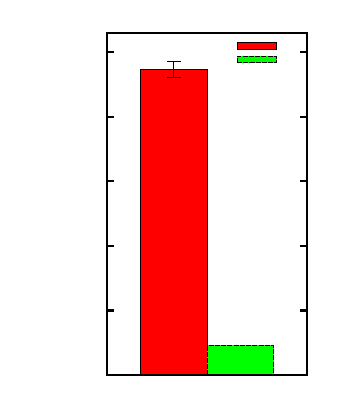
\includegraphics{CumulativeSumRankL2CHits}}%
    \gplfronttext
  \end{picture}%
\endgroup

\caption{Level 2 Cache Hits}
\label{fig:CumulativeSumRankL2CHits}
\end{subfigure}
\hfill
%\begin{subfigure}{0.30\textwidth}
%	% GNUPLOT: LaTeX picture with Postscript
\begingroup
  \makeatletter
  \providecommand\color[2][]{%
    \GenericError{(gnuplot) \space\space\space\@spaces}{%
      Package color not loaded in conjunction with
      terminal option `colourtext'%
    }{See the gnuplot documentation for explanation.%
    }{Either use 'blacktext' in gnuplot or load the package
      color.sty in LaTeX.}%
    \renewcommand\color[2][]{}%
  }%
  \providecommand\includegraphics[2][]{%
    \GenericError{(gnuplot) \space\space\space\@spaces}{%
      Package graphicx or graphics not loaded%
    }{See the gnuplot documentation for explanation.%
    }{The gnuplot epslatex terminal needs graphicx.sty or graphics.sty.}%
    \renewcommand\includegraphics[2][]{}%
  }%
  \providecommand\rotatebox[2]{#2}%
  \@ifundefined{ifGPcolor}{%
    \newif\ifGPcolor
    \GPcolortrue
  }{}%
  \@ifundefined{ifGPblacktext}{%
    \newif\ifGPblacktext
    \GPblacktexttrue
  }{}%
  % define a \g@addto@macro without @ in the name:
  \let\gplgaddtomacro\g@addto@macro
  % define empty templates for all commands taking text:
  \gdef\gplbacktext{}%
  \gdef\gplfronttext{}%
  \makeatother
  \ifGPblacktext
    % no textcolor at all
    \def\colorrgb#1{}%
    \def\colorgray#1{}%
  \else
    % gray or color?
    \ifGPcolor
      \def\colorrgb#1{\color[rgb]{#1}}%
      \def\colorgray#1{\color[gray]{#1}}%
      \expandafter\def\csname LTw\endcsname{\color{white}}%
      \expandafter\def\csname LTb\endcsname{\color{black}}%
      \expandafter\def\csname LTa\endcsname{\color{black}}%
      \expandafter\def\csname LT0\endcsname{\color[rgb]{1,0,0}}%
      \expandafter\def\csname LT1\endcsname{\color[rgb]{0,1,0}}%
      \expandafter\def\csname LT2\endcsname{\color[rgb]{0,0,1}}%
      \expandafter\def\csname LT3\endcsname{\color[rgb]{1,0,1}}%
      \expandafter\def\csname LT4\endcsname{\color[rgb]{0,1,1}}%
      \expandafter\def\csname LT5\endcsname{\color[rgb]{1,1,0}}%
      \expandafter\def\csname LT6\endcsname{\color[rgb]{0,0,0}}%
      \expandafter\def\csname LT7\endcsname{\color[rgb]{1,0.3,0}}%
      \expandafter\def\csname LT8\endcsname{\color[rgb]{0.5,0.5,0.5}}%
    \else
      % gray
      \def\colorrgb#1{\color{black}}%
      \def\colorgray#1{\color[gray]{#1}}%
      \expandafter\def\csname LTw\endcsname{\color{white}}%
      \expandafter\def\csname LTb\endcsname{\color{black}}%
      \expandafter\def\csname LTa\endcsname{\color{black}}%
      \expandafter\def\csname LT0\endcsname{\color{black}}%
      \expandafter\def\csname LT1\endcsname{\color{black}}%
      \expandafter\def\csname LT2\endcsname{\color{black}}%
      \expandafter\def\csname LT3\endcsname{\color{black}}%
      \expandafter\def\csname LT4\endcsname{\color{black}}%
      \expandafter\def\csname LT5\endcsname{\color{black}}%
      \expandafter\def\csname LT6\endcsname{\color{black}}%
      \expandafter\def\csname LT7\endcsname{\color{black}}%
      \expandafter\def\csname LT8\endcsname{\color{black}}%
    \fi
  \fi
  \setlength{\unitlength}{0.0500bp}%
  \begin{picture}(3024.00,3600.00)%
    \gplgaddtomacro\gplbacktext{%
      \csname LTb\endcsname%
      \put(559,156){\makebox(0,0)[r]{\strut{} 0}}%
      \put(559,978){\makebox(0,0)[r]{\strut{} 0.5}}%
      \put(559,1800){\makebox(0,0)[r]{\strut{} 1}}%
      \put(559,2621){\makebox(0,0)[r]{\strut{} 1.5}}%
      \put(559,3443){\makebox(0,0)[r]{\strut{} 2}}%
      \put(104,1799){\rotatebox{-270}{\makebox(0,0){\strut{}Cache Miss Rate}}}%
    }%
    \gplgaddtomacro\gplfronttext{%
      \csname LTb\endcsname%
      \put(1807,3315){\makebox(0,0)[r]{\strut{}UnalignedNaive}}%
      \csname LTb\endcsname%
      \put(1807,3185){\makebox(0,0)[r]{\strut{}CumulativeSum}}%
    }%
    \gplbacktext
    \put(0,0){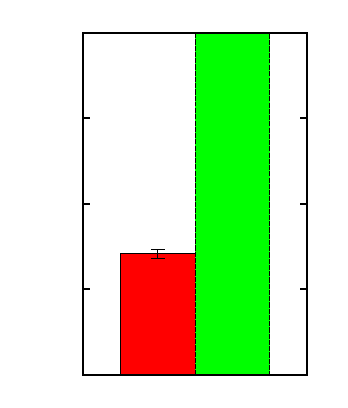
\includegraphics{CumulativeSumRankL2CMRate}}%
    \gplfronttext
  \end{picture}%
\endgroup

%	\caption{Level 2 Cache Miss Rate}
%	\label{fig:CumulativeSumRankL2CMRate}
%\end{subfigure}
%\hfill
\begin{subfigure}{0.30\textwidth}
	% GNUPLOT: LaTeX picture with Postscript
\begingroup
  \makeatletter
  \providecommand\color[2][]{%
    \GenericError{(gnuplot) \space\space\space\@spaces}{%
      Package color not loaded in conjunction with
      terminal option `colourtext'%
    }{See the gnuplot documentation for explanation.%
    }{Either use 'blacktext' in gnuplot or load the package
      color.sty in LaTeX.}%
    \renewcommand\color[2][]{}%
  }%
  \providecommand\includegraphics[2][]{%
    \GenericError{(gnuplot) \space\space\space\@spaces}{%
      Package graphicx or graphics not loaded%
    }{See the gnuplot documentation for explanation.%
    }{The gnuplot epslatex terminal needs graphicx.sty or graphics.sty.}%
    \renewcommand\includegraphics[2][]{}%
  }%
  \providecommand\rotatebox[2]{#2}%
  \@ifundefined{ifGPcolor}{%
    \newif\ifGPcolor
    \GPcolortrue
  }{}%
  \@ifundefined{ifGPblacktext}{%
    \newif\ifGPblacktext
    \GPblacktexttrue
  }{}%
  % define a \g@addto@macro without @ in the name:
  \let\gplgaddtomacro\g@addto@macro
  % define empty templates for all commands taking text:
  \gdef\gplbacktext{}%
  \gdef\gplfronttext{}%
  \makeatother
  \ifGPblacktext
    % no textcolor at all
    \def\colorrgb#1{}%
    \def\colorgray#1{}%
  \else
    % gray or color?
    \ifGPcolor
      \def\colorrgb#1{\color[rgb]{#1}}%
      \def\colorgray#1{\color[gray]{#1}}%
      \expandafter\def\csname LTw\endcsname{\color{white}}%
      \expandafter\def\csname LTb\endcsname{\color{black}}%
      \expandafter\def\csname LTa\endcsname{\color{black}}%
      \expandafter\def\csname LT0\endcsname{\color[rgb]{1,0,0}}%
      \expandafter\def\csname LT1\endcsname{\color[rgb]{0,1,0}}%
      \expandafter\def\csname LT2\endcsname{\color[rgb]{0,0,1}}%
      \expandafter\def\csname LT3\endcsname{\color[rgb]{1,0,1}}%
      \expandafter\def\csname LT4\endcsname{\color[rgb]{0,1,1}}%
      \expandafter\def\csname LT5\endcsname{\color[rgb]{1,1,0}}%
      \expandafter\def\csname LT6\endcsname{\color[rgb]{0,0,0}}%
      \expandafter\def\csname LT7\endcsname{\color[rgb]{1,0.3,0}}%
      \expandafter\def\csname LT8\endcsname{\color[rgb]{0.5,0.5,0.5}}%
    \else
      % gray
      \def\colorrgb#1{\color{black}}%
      \def\colorgray#1{\color[gray]{#1}}%
      \expandafter\def\csname LTw\endcsname{\color{white}}%
      \expandafter\def\csname LTb\endcsname{\color{black}}%
      \expandafter\def\csname LTa\endcsname{\color{black}}%
      \expandafter\def\csname LT0\endcsname{\color{black}}%
      \expandafter\def\csname LT1\endcsname{\color{black}}%
      \expandafter\def\csname LT2\endcsname{\color{black}}%
      \expandafter\def\csname LT3\endcsname{\color{black}}%
      \expandafter\def\csname LT4\endcsname{\color{black}}%
      \expandafter\def\csname LT5\endcsname{\color{black}}%
      \expandafter\def\csname LT6\endcsname{\color{black}}%
      \expandafter\def\csname LT7\endcsname{\color{black}}%
      \expandafter\def\csname LT8\endcsname{\color{black}}%
    \fi
  \fi
  \setlength{\unitlength}{0.0500bp}%
  \begin{picture}(3024.00,3600.00)%
    \gplgaddtomacro\gplbacktext{%
      \csname LTb\endcsname%
      \put(793,156){\makebox(0,0)[r]{\strut{} 0}}%
      \put(793,567){\makebox(0,0)[r]{\strut{} 20000}}%
      \put(793,978){\makebox(0,0)[r]{\strut{} 40000}}%
      \put(793,1389){\makebox(0,0)[r]{\strut{} 60000}}%
      \put(793,1800){\makebox(0,0)[r]{\strut{} 80000}}%
      \put(793,2210){\makebox(0,0)[r]{\strut{} 100000}}%
      \put(793,2621){\makebox(0,0)[r]{\strut{} 120000}}%
      \put(793,3032){\makebox(0,0)[r]{\strut{} 140000}}%
      \put(793,3443){\makebox(0,0)[r]{\strut{} 160000}}%
      \put(104,1799){\rotatebox{-270}{\makebox(0,0){\strut{}Cache Misses}}}%
    }%
    \gplgaddtomacro\gplfronttext{%
      \csname LTb\endcsname%
      \put(2041,3315){\makebox(0,0)[r]{\strut{}UnalignedNaive}}%
      \csname LTb\endcsname%
      \put(2041,3185){\makebox(0,0)[r]{\strut{}CumulativeSum}}%
    }%
    \gplbacktext
    \put(0,0){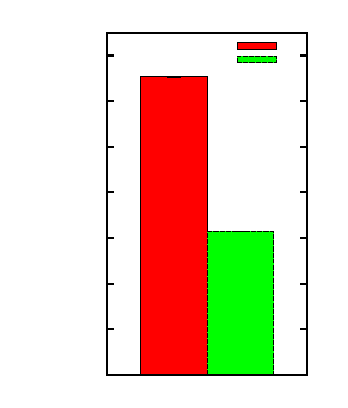
\includegraphics{CumulativeSumRankL3CM}}%
    \gplfronttext
  \end{picture}%
\endgroup

	\caption{Level 3 Cache Misses}
	\label{fig:CumulativeSumRankL3CM}
\end{subfigure}

\caption{Measurements on Rank Queries on the UnalignedNaive and CumulativeSum Wavelet Trees. Part 1.}
\label{fig:CumulativeSumRank}
\end{figure}





\clearpage




\begin{figure}\tiny

\begin{subfigure}{0.30\textwidth}
	% GNUPLOT: LaTeX picture with Postscript
\begingroup
  \makeatletter
  \providecommand\color[2][]{%
    \GenericError{(gnuplot) \space\space\space\@spaces}{%
      Package color not loaded in conjunction with
      terminal option `colourtext'%
    }{See the gnuplot documentation for explanation.%
    }{Either use 'blacktext' in gnuplot or load the package
      color.sty in LaTeX.}%
    \renewcommand\color[2][]{}%
  }%
  \providecommand\includegraphics[2][]{%
    \GenericError{(gnuplot) \space\space\space\@spaces}{%
      Package graphicx or graphics not loaded%
    }{See the gnuplot documentation for explanation.%
    }{The gnuplot epslatex terminal needs graphicx.sty or graphics.sty.}%
    \renewcommand\includegraphics[2][]{}%
  }%
  \providecommand\rotatebox[2]{#2}%
  \@ifundefined{ifGPcolor}{%
    \newif\ifGPcolor
    \GPcolortrue
  }{}%
  \@ifundefined{ifGPblacktext}{%
    \newif\ifGPblacktext
    \GPblacktexttrue
  }{}%
  % define a \g@addto@macro without @ in the name:
  \let\gplgaddtomacro\g@addto@macro
  % define empty templates for all commands taking text:
  \gdef\gplbacktext{}%
  \gdef\gplfronttext{}%
  \makeatother
  \ifGPblacktext
    % no textcolor at all
    \def\colorrgb#1{}%
    \def\colorgray#1{}%
  \else
    % gray or color?
    \ifGPcolor
      \def\colorrgb#1{\color[rgb]{#1}}%
      \def\colorgray#1{\color[gray]{#1}}%
      \expandafter\def\csname LTw\endcsname{\color{white}}%
      \expandafter\def\csname LTb\endcsname{\color{black}}%
      \expandafter\def\csname LTa\endcsname{\color{black}}%
      \expandafter\def\csname LT0\endcsname{\color[rgb]{1,0,0}}%
      \expandafter\def\csname LT1\endcsname{\color[rgb]{0,1,0}}%
      \expandafter\def\csname LT2\endcsname{\color[rgb]{0,0,1}}%
      \expandafter\def\csname LT3\endcsname{\color[rgb]{1,0,1}}%
      \expandafter\def\csname LT4\endcsname{\color[rgb]{0,1,1}}%
      \expandafter\def\csname LT5\endcsname{\color[rgb]{1,1,0}}%
      \expandafter\def\csname LT6\endcsname{\color[rgb]{0,0,0}}%
      \expandafter\def\csname LT7\endcsname{\color[rgb]{1,0.3,0}}%
      \expandafter\def\csname LT8\endcsname{\color[rgb]{0.5,0.5,0.5}}%
    \else
      % gray
      \def\colorrgb#1{\color{black}}%
      \def\colorgray#1{\color[gray]{#1}}%
      \expandafter\def\csname LTw\endcsname{\color{white}}%
      \expandafter\def\csname LTb\endcsname{\color{black}}%
      \expandafter\def\csname LTa\endcsname{\color{black}}%
      \expandafter\def\csname LT0\endcsname{\color{black}}%
      \expandafter\def\csname LT1\endcsname{\color{black}}%
      \expandafter\def\csname LT2\endcsname{\color{black}}%
      \expandafter\def\csname LT3\endcsname{\color{black}}%
      \expandafter\def\csname LT4\endcsname{\color{black}}%
      \expandafter\def\csname LT5\endcsname{\color{black}}%
      \expandafter\def\csname LT6\endcsname{\color{black}}%
      \expandafter\def\csname LT7\endcsname{\color{black}}%
      \expandafter\def\csname LT8\endcsname{\color{black}}%
    \fi
  \fi
  \setlength{\unitlength}{0.0500bp}%
  \begin{picture}(3024.00,3600.00)%
    \gplgaddtomacro\gplbacktext{%
      \csname LTb\endcsname%
      \put(481,156){\makebox(0,0)[r]{\strut{} 0}}%
      \put(481,626){\makebox(0,0)[r]{\strut{} 2}}%
      \put(481,1095){\makebox(0,0)[r]{\strut{} 4}}%
      \put(481,1565){\makebox(0,0)[r]{\strut{} 6}}%
      \put(481,2034){\makebox(0,0)[r]{\strut{} 8}}%
      \put(481,2504){\makebox(0,0)[r]{\strut{} 10}}%
      \put(481,2973){\makebox(0,0)[r]{\strut{} 12}}%
      \put(481,3443){\makebox(0,0)[r]{\strut{} 14}}%
      \put(104,1799){\rotatebox{-270}{\makebox(0,0){\strut{}Walltime (milliseconds)}}}%
    }%
    \gplgaddtomacro\gplfronttext{%
      \csname LTb\endcsname%
      \put(2180,3315){\makebox(0,0)[r]{\strut{}UnalignedNaive}}%
      \csname LTb\endcsname%
      \put(2180,3185){\makebox(0,0)[r]{\strut{}CumulativeSum}}%
      \csname LTb\endcsname%
      \put(2180,3055){\makebox(0,0)[r]{\strut{}CumSumBranchless}}%
    }%
    \gplbacktext
    \put(0,0){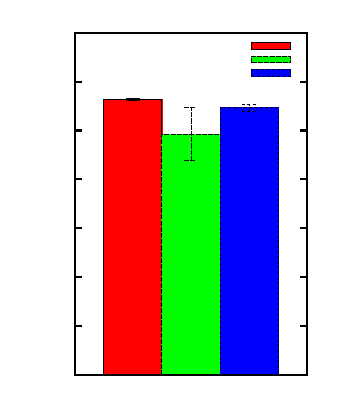
\includegraphics{CumulativeSumSelectWalltime}}%
    \gplfronttext
  \end{picture}%
\endgroup

	\caption{Wall Time}
	\label{fig:CumulativeSumSelectWalltime}
\end{subfigure}
\hfill
\begin{subfigure}{0.30\textwidth}
	% GNUPLOT: LaTeX picture with Postscript
\begingroup
  \makeatletter
  \providecommand\color[2][]{%
    \GenericError{(gnuplot) \space\space\space\@spaces}{%
      Package color not loaded in conjunction with
      terminal option `colourtext'%
    }{See the gnuplot documentation for explanation.%
    }{Either use 'blacktext' in gnuplot or load the package
      color.sty in LaTeX.}%
    \renewcommand\color[2][]{}%
  }%
  \providecommand\includegraphics[2][]{%
    \GenericError{(gnuplot) \space\space\space\@spaces}{%
      Package graphicx or graphics not loaded%
    }{See the gnuplot documentation for explanation.%
    }{The gnuplot epslatex terminal needs graphicx.sty or graphics.sty.}%
    \renewcommand\includegraphics[2][]{}%
  }%
  \providecommand\rotatebox[2]{#2}%
  \@ifundefined{ifGPcolor}{%
    \newif\ifGPcolor
    \GPcolortrue
  }{}%
  \@ifundefined{ifGPblacktext}{%
    \newif\ifGPblacktext
    \GPblacktexttrue
  }{}%
  % define a \g@addto@macro without @ in the name:
  \let\gplgaddtomacro\g@addto@macro
  % define empty templates for all commands taking text:
  \gdef\gplbacktext{}%
  \gdef\gplfronttext{}%
  \makeatother
  \ifGPblacktext
    % no textcolor at all
    \def\colorrgb#1{}%
    \def\colorgray#1{}%
  \else
    % gray or color?
    \ifGPcolor
      \def\colorrgb#1{\color[rgb]{#1}}%
      \def\colorgray#1{\color[gray]{#1}}%
      \expandafter\def\csname LTw\endcsname{\color{white}}%
      \expandafter\def\csname LTb\endcsname{\color{black}}%
      \expandafter\def\csname LTa\endcsname{\color{black}}%
      \expandafter\def\csname LT0\endcsname{\color[rgb]{1,0,0}}%
      \expandafter\def\csname LT1\endcsname{\color[rgb]{0,1,0}}%
      \expandafter\def\csname LT2\endcsname{\color[rgb]{0,0,1}}%
      \expandafter\def\csname LT3\endcsname{\color[rgb]{1,0,1}}%
      \expandafter\def\csname LT4\endcsname{\color[rgb]{0,1,1}}%
      \expandafter\def\csname LT5\endcsname{\color[rgb]{1,1,0}}%
      \expandafter\def\csname LT6\endcsname{\color[rgb]{0,0,0}}%
      \expandafter\def\csname LT7\endcsname{\color[rgb]{1,0.3,0}}%
      \expandafter\def\csname LT8\endcsname{\color[rgb]{0.5,0.5,0.5}}%
    \else
      % gray
      \def\colorrgb#1{\color{black}}%
      \def\colorgray#1{\color[gray]{#1}}%
      \expandafter\def\csname LTw\endcsname{\color{white}}%
      \expandafter\def\csname LTb\endcsname{\color{black}}%
      \expandafter\def\csname LTa\endcsname{\color{black}}%
      \expandafter\def\csname LT0\endcsname{\color{black}}%
      \expandafter\def\csname LT1\endcsname{\color{black}}%
      \expandafter\def\csname LT2\endcsname{\color{black}}%
      \expandafter\def\csname LT3\endcsname{\color{black}}%
      \expandafter\def\csname LT4\endcsname{\color{black}}%
      \expandafter\def\csname LT5\endcsname{\color{black}}%
      \expandafter\def\csname LT6\endcsname{\color{black}}%
      \expandafter\def\csname LT7\endcsname{\color{black}}%
      \expandafter\def\csname LT8\endcsname{\color{black}}%
    \fi
  \fi
  \setlength{\unitlength}{0.0500bp}%
  \begin{picture}(4608.00,3600.00)%
    \gplgaddtomacro\gplbacktext{%
      \csname LTb\endcsname%
      \put(793,156){\makebox(0,0)[r]{\strut{} 0}}%
      \put(793,567){\makebox(0,0)[r]{\strut{} 50000}}%
      \put(793,978){\makebox(0,0)[r]{\strut{} 100000}}%
      \put(793,1389){\makebox(0,0)[r]{\strut{} 150000}}%
      \put(793,1800){\makebox(0,0)[r]{\strut{} 200000}}%
      \put(793,2210){\makebox(0,0)[r]{\strut{} 250000}}%
      \put(793,2621){\makebox(0,0)[r]{\strut{} 300000}}%
      \put(793,3032){\makebox(0,0)[r]{\strut{} 350000}}%
      \put(793,3443){\makebox(0,0)[r]{\strut{} 400000}}%
      \put(104,1799){\rotatebox{-270}{\makebox(0,0){\strut{}Branch Misses}}}%
    }%
    \gplgaddtomacro\gplfronttext{%
      \csname LTb\endcsname%
      \put(1985,3315){\makebox(0,0)[r]{\strut{}UnalignedNaive}}%
      \csname LTb\endcsname%
      \put(1985,3185){\makebox(0,0)[r]{\strut{}CumulativeSum}}%
      \csname LTb\endcsname%
      \put(3764,3315){\makebox(0,0)[r]{\strut{}CumSumBranchless}}%
    }%
    \gplbacktext
    \put(0,0){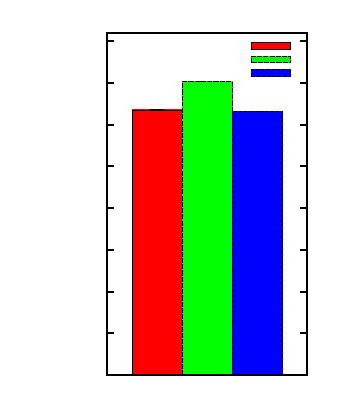
\includegraphics{CumulativeSumSelectBranchMiss}}%
    \gplfronttext
  \end{picture}%
\endgroup

	\caption{Branch Mispredictions}
	\label{fig:CumulativeSumSelectBranchMiss}
\end{subfigure}
\hfill
\begin{subfigure}{0.30\textwidth}
	% GNUPLOT: LaTeX picture with Postscript
\begingroup
  \makeatletter
  \providecommand\color[2][]{%
    \GenericError{(gnuplot) \space\space\space\@spaces}{%
      Package color not loaded in conjunction with
      terminal option `colourtext'%
    }{See the gnuplot documentation for explanation.%
    }{Either use 'blacktext' in gnuplot or load the package
      color.sty in LaTeX.}%
    \renewcommand\color[2][]{}%
  }%
  \providecommand\includegraphics[2][]{%
    \GenericError{(gnuplot) \space\space\space\@spaces}{%
      Package graphicx or graphics not loaded%
    }{See the gnuplot documentation for explanation.%
    }{The gnuplot epslatex terminal needs graphicx.sty or graphics.sty.}%
    \renewcommand\includegraphics[2][]{}%
  }%
  \providecommand\rotatebox[2]{#2}%
  \@ifundefined{ifGPcolor}{%
    \newif\ifGPcolor
    \GPcolortrue
  }{}%
  \@ifundefined{ifGPblacktext}{%
    \newif\ifGPblacktext
    \GPblacktexttrue
  }{}%
  % define a \g@addto@macro without @ in the name:
  \let\gplgaddtomacro\g@addto@macro
  % define empty templates for all commands taking text:
  \gdef\gplbacktext{}%
  \gdef\gplfronttext{}%
  \makeatother
  \ifGPblacktext
    % no textcolor at all
    \def\colorrgb#1{}%
    \def\colorgray#1{}%
  \else
    % gray or color?
    \ifGPcolor
      \def\colorrgb#1{\color[rgb]{#1}}%
      \def\colorgray#1{\color[gray]{#1}}%
      \expandafter\def\csname LTw\endcsname{\color{white}}%
      \expandafter\def\csname LTb\endcsname{\color{black}}%
      \expandafter\def\csname LTa\endcsname{\color{black}}%
      \expandafter\def\csname LT0\endcsname{\color[rgb]{1,0,0}}%
      \expandafter\def\csname LT1\endcsname{\color[rgb]{0,1,0}}%
      \expandafter\def\csname LT2\endcsname{\color[rgb]{0,0,1}}%
      \expandafter\def\csname LT3\endcsname{\color[rgb]{1,0,1}}%
      \expandafter\def\csname LT4\endcsname{\color[rgb]{0,1,1}}%
      \expandafter\def\csname LT5\endcsname{\color[rgb]{1,1,0}}%
      \expandafter\def\csname LT6\endcsname{\color[rgb]{0,0,0}}%
      \expandafter\def\csname LT7\endcsname{\color[rgb]{1,0.3,0}}%
      \expandafter\def\csname LT8\endcsname{\color[rgb]{0.5,0.5,0.5}}%
    \else
      % gray
      \def\colorrgb#1{\color{black}}%
      \def\colorgray#1{\color[gray]{#1}}%
      \expandafter\def\csname LTw\endcsname{\color{white}}%
      \expandafter\def\csname LTb\endcsname{\color{black}}%
      \expandafter\def\csname LTa\endcsname{\color{black}}%
      \expandafter\def\csname LT0\endcsname{\color{black}}%
      \expandafter\def\csname LT1\endcsname{\color{black}}%
      \expandafter\def\csname LT2\endcsname{\color{black}}%
      \expandafter\def\csname LT3\endcsname{\color{black}}%
      \expandafter\def\csname LT4\endcsname{\color{black}}%
      \expandafter\def\csname LT5\endcsname{\color{black}}%
      \expandafter\def\csname LT6\endcsname{\color{black}}%
      \expandafter\def\csname LT7\endcsname{\color{black}}%
      \expandafter\def\csname LT8\endcsname{\color{black}}%
    \fi
  \fi
  \setlength{\unitlength}{0.0500bp}%
  \begin{picture}(3024.00,3600.00)%
    \gplgaddtomacro\gplbacktext{%
      \csname LTb\endcsname%
      \put(871,156){\makebox(0,0)[r]{\strut{} 0}}%
      \put(871,594){\makebox(0,0)[r]{\strut{} 2e+06}}%
      \put(871,1033){\makebox(0,0)[r]{\strut{} 4e+06}}%
      \put(871,1471){\makebox(0,0)[r]{\strut{} 6e+06}}%
      \put(871,1909){\makebox(0,0)[r]{\strut{} 8e+06}}%
      \put(871,2347){\makebox(0,0)[r]{\strut{} 1e+07}}%
      \put(871,2786){\makebox(0,0)[r]{\strut{} 1.2e+07}}%
      \put(871,3224){\makebox(0,0)[r]{\strut{} 1.4e+07}}%
      \put(104,1799){\rotatebox{-270}{\makebox(0,0){\strut{}Branches Executed}}}%
    }%
    \gplgaddtomacro\gplfronttext{%
      \csname LTb\endcsname%
      \put(2180,3315){\makebox(0,0)[r]{\strut{}UnalignedNaive}}%
      \csname LTb\endcsname%
      \put(2180,3185){\makebox(0,0)[r]{\strut{}CumulativeSum}}%
      \csname LTb\endcsname%
      \put(2180,3055){\makebox(0,0)[r]{\strut{}CumSumBranchless}}%
    }%
    \gplbacktext
    \put(0,0){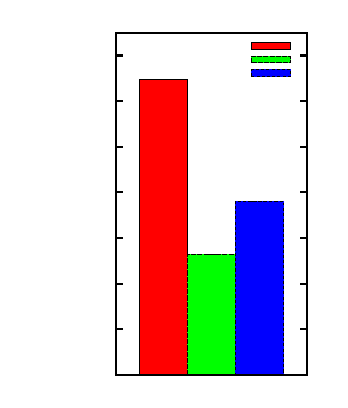
\includegraphics{CumulativeSumSelectBranchExe}}%
    \gplfronttext
  \end{picture}%
\endgroup

	\caption{Branches Executed}
	\label{fig:CumulativeSumSelectBranchExe}
\end{subfigure}


\begin{subfigure}{0.30\textwidth}
	% GNUPLOT: LaTeX picture with Postscript
\begingroup
  \makeatletter
  \providecommand\color[2][]{%
    \GenericError{(gnuplot) \space\space\space\@spaces}{%
      Package color not loaded in conjunction with
      terminal option `colourtext'%
    }{See the gnuplot documentation for explanation.%
    }{Either use 'blacktext' in gnuplot or load the package
      color.sty in LaTeX.}%
    \renewcommand\color[2][]{}%
  }%
  \providecommand\includegraphics[2][]{%
    \GenericError{(gnuplot) \space\space\space\@spaces}{%
      Package graphicx or graphics not loaded%
    }{See the gnuplot documentation for explanation.%
    }{The gnuplot epslatex terminal needs graphicx.sty or graphics.sty.}%
    \renewcommand\includegraphics[2][]{}%
  }%
  \providecommand\rotatebox[2]{#2}%
  \@ifundefined{ifGPcolor}{%
    \newif\ifGPcolor
    \GPcolortrue
  }{}%
  \@ifundefined{ifGPblacktext}{%
    \newif\ifGPblacktext
    \GPblacktexttrue
  }{}%
  % define a \g@addto@macro without @ in the name:
  \let\gplgaddtomacro\g@addto@macro
  % define empty templates for all commands taking text:
  \gdef\gplbacktext{}%
  \gdef\gplfronttext{}%
  \makeatother
  \ifGPblacktext
    % no textcolor at all
    \def\colorrgb#1{}%
    \def\colorgray#1{}%
  \else
    % gray or color?
    \ifGPcolor
      \def\colorrgb#1{\color[rgb]{#1}}%
      \def\colorgray#1{\color[gray]{#1}}%
      \expandafter\def\csname LTw\endcsname{\color{white}}%
      \expandafter\def\csname LTb\endcsname{\color{black}}%
      \expandafter\def\csname LTa\endcsname{\color{black}}%
      \expandafter\def\csname LT0\endcsname{\color[rgb]{1,0,0}}%
      \expandafter\def\csname LT1\endcsname{\color[rgb]{0,1,0}}%
      \expandafter\def\csname LT2\endcsname{\color[rgb]{0,0,1}}%
      \expandafter\def\csname LT3\endcsname{\color[rgb]{1,0,1}}%
      \expandafter\def\csname LT4\endcsname{\color[rgb]{0,1,1}}%
      \expandafter\def\csname LT5\endcsname{\color[rgb]{1,1,0}}%
      \expandafter\def\csname LT6\endcsname{\color[rgb]{0,0,0}}%
      \expandafter\def\csname LT7\endcsname{\color[rgb]{1,0.3,0}}%
      \expandafter\def\csname LT8\endcsname{\color[rgb]{0.5,0.5,0.5}}%
    \else
      % gray
      \def\colorrgb#1{\color{black}}%
      \def\colorgray#1{\color[gray]{#1}}%
      \expandafter\def\csname LTw\endcsname{\color{white}}%
      \expandafter\def\csname LTb\endcsname{\color{black}}%
      \expandafter\def\csname LTa\endcsname{\color{black}}%
      \expandafter\def\csname LT0\endcsname{\color{black}}%
      \expandafter\def\csname LT1\endcsname{\color{black}}%
      \expandafter\def\csname LT2\endcsname{\color{black}}%
      \expandafter\def\csname LT3\endcsname{\color{black}}%
      \expandafter\def\csname LT4\endcsname{\color{black}}%
      \expandafter\def\csname LT5\endcsname{\color{black}}%
      \expandafter\def\csname LT6\endcsname{\color{black}}%
      \expandafter\def\csname LT7\endcsname{\color{black}}%
      \expandafter\def\csname LT8\endcsname{\color{black}}%
    \fi
  \fi
  \setlength{\unitlength}{0.0500bp}%
  \begin{picture}(3024.00,3600.00)%
    \gplgaddtomacro\gplbacktext{%
      \csname LTb\endcsname%
      \put(637,156){\makebox(0,0)[r]{\strut{} 0}}%
      \put(637,978){\makebox(0,0)[r]{\strut{} 0.05}}%
      \put(637,1800){\makebox(0,0)[r]{\strut{} 0.1}}%
      \put(637,2621){\makebox(0,0)[r]{\strut{} 0.15}}%
      \put(637,3443){\makebox(0,0)[r]{\strut{} 0.2}}%
      \put(104,1799){\rotatebox{-270}{\makebox(0,0){\strut{}Branch Misprediction Rate}}}%
    }%
    \gplgaddtomacro\gplfronttext{%
      \csname LTb\endcsname%
      \put(2180,3315){\makebox(0,0)[r]{\strut{}UnalignedNaive}}%
      \csname LTb\endcsname%
      \put(2180,3185){\makebox(0,0)[r]{\strut{}CumulativeSum}}%
      \csname LTb\endcsname%
      \put(2180,3055){\makebox(0,0)[r]{\strut{}CumSumBranchless}}%
    }%
    \gplbacktext
    \put(0,0){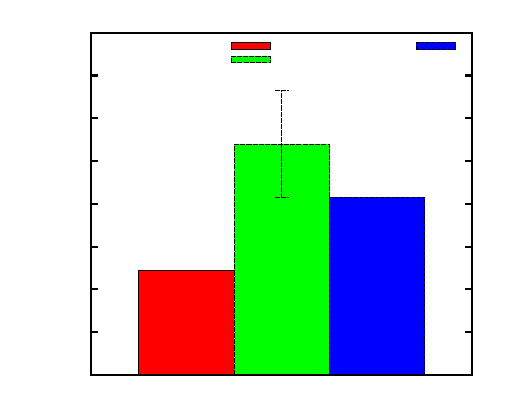
\includegraphics{CumulativeSumSelectBranchMissRate}}%
    \gplfronttext
  \end{picture}%
\endgroup

	\caption{Branch Misprediction Rate}
	\label{fig:CumulativeSumSelectBranchMissRate}
\end{subfigure}
\hfill
\begin{subfigure}{0.30\textwidth}
	% GNUPLOT: LaTeX picture with Postscript
\begingroup
  \makeatletter
  \providecommand\color[2][]{%
    \GenericError{(gnuplot) \space\space\space\@spaces}{%
      Package color not loaded in conjunction with
      terminal option `colourtext'%
    }{See the gnuplot documentation for explanation.%
    }{Either use 'blacktext' in gnuplot or load the package
      color.sty in LaTeX.}%
    \renewcommand\color[2][]{}%
  }%
  \providecommand\includegraphics[2][]{%
    \GenericError{(gnuplot) \space\space\space\@spaces}{%
      Package graphicx or graphics not loaded%
    }{See the gnuplot documentation for explanation.%
    }{The gnuplot epslatex terminal needs graphicx.sty or graphics.sty.}%
    \renewcommand\includegraphics[2][]{}%
  }%
  \providecommand\rotatebox[2]{#2}%
  \@ifundefined{ifGPcolor}{%
    \newif\ifGPcolor
    \GPcolortrue
  }{}%
  \@ifundefined{ifGPblacktext}{%
    \newif\ifGPblacktext
    \GPblacktexttrue
  }{}%
  % define a \g@addto@macro without @ in the name:
  \let\gplgaddtomacro\g@addto@macro
  % define empty templates for all commands taking text:
  \gdef\gplbacktext{}%
  \gdef\gplfronttext{}%
  \makeatother
  \ifGPblacktext
    % no textcolor at all
    \def\colorrgb#1{}%
    \def\colorgray#1{}%
  \else
    % gray or color?
    \ifGPcolor
      \def\colorrgb#1{\color[rgb]{#1}}%
      \def\colorgray#1{\color[gray]{#1}}%
      \expandafter\def\csname LTw\endcsname{\color{white}}%
      \expandafter\def\csname LTb\endcsname{\color{black}}%
      \expandafter\def\csname LTa\endcsname{\color{black}}%
      \expandafter\def\csname LT0\endcsname{\color[rgb]{1,0,0}}%
      \expandafter\def\csname LT1\endcsname{\color[rgb]{0,1,0}}%
      \expandafter\def\csname LT2\endcsname{\color[rgb]{0,0,1}}%
      \expandafter\def\csname LT3\endcsname{\color[rgb]{1,0,1}}%
      \expandafter\def\csname LT4\endcsname{\color[rgb]{0,1,1}}%
      \expandafter\def\csname LT5\endcsname{\color[rgb]{1,1,0}}%
      \expandafter\def\csname LT6\endcsname{\color[rgb]{0,0,0}}%
      \expandafter\def\csname LT7\endcsname{\color[rgb]{1,0.3,0}}%
      \expandafter\def\csname LT8\endcsname{\color[rgb]{0.5,0.5,0.5}}%
    \else
      % gray
      \def\colorrgb#1{\color{black}}%
      \def\colorgray#1{\color[gray]{#1}}%
      \expandafter\def\csname LTw\endcsname{\color{white}}%
      \expandafter\def\csname LTb\endcsname{\color{black}}%
      \expandafter\def\csname LTa\endcsname{\color{black}}%
      \expandafter\def\csname LT0\endcsname{\color{black}}%
      \expandafter\def\csname LT1\endcsname{\color{black}}%
      \expandafter\def\csname LT2\endcsname{\color{black}}%
      \expandafter\def\csname LT3\endcsname{\color{black}}%
      \expandafter\def\csname LT4\endcsname{\color{black}}%
      \expandafter\def\csname LT5\endcsname{\color{black}}%
      \expandafter\def\csname LT6\endcsname{\color{black}}%
      \expandafter\def\csname LT7\endcsname{\color{black}}%
      \expandafter\def\csname LT8\endcsname{\color{black}}%
    \fi
  \fi
  \setlength{\unitlength}{0.0500bp}%
  \begin{picture}(3024.00,3600.00)%
    \gplgaddtomacro\gplbacktext{%
      \csname LTb\endcsname%
      \put(637,156){\makebox(0,0)[r]{\strut{} 0}}%
      \put(637,521){\makebox(0,0)[r]{\strut{} 1000}}%
      \put(637,886){\makebox(0,0)[r]{\strut{} 2000}}%
      \put(637,1252){\makebox(0,0)[r]{\strut{} 3000}}%
      \put(637,1617){\makebox(0,0)[r]{\strut{} 4000}}%
      \put(637,1982){\makebox(0,0)[r]{\strut{} 5000}}%
      \put(637,2347){\makebox(0,0)[r]{\strut{} 6000}}%
      \put(637,2713){\makebox(0,0)[r]{\strut{} 7000}}%
      \put(637,3078){\makebox(0,0)[r]{\strut{} 8000}}%
      \put(637,3443){\makebox(0,0)[r]{\strut{} 9000}}%
      \put(104,1799){\rotatebox{-270}{\makebox(0,0){\strut{}TLB Misses}}}%
    }%
    \gplgaddtomacro\gplfronttext{%
      \csname LTb\endcsname%
      \put(2180,3315){\makebox(0,0)[r]{\strut{}UnalignedNaive}}%
      \csname LTb\endcsname%
      \put(2180,3185){\makebox(0,0)[r]{\strut{}CumulativeSum}}%
      \csname LTb\endcsname%
      \put(2180,3055){\makebox(0,0)[r]{\strut{}CumSumBranchless}}%
    }%
    \gplbacktext
    \put(0,0){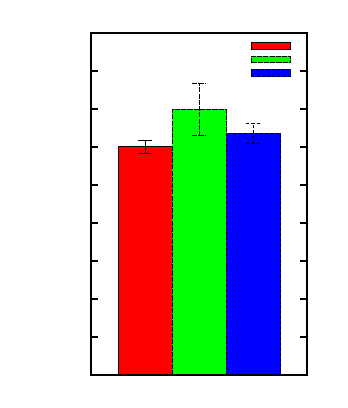
\includegraphics{CumulativeSumSelectTLBMiss}}%
    \gplfronttext
  \end{picture}%
\endgroup

	\caption{TLB Misses}
	\label{fig:CumulativeSumSelectTLBMiss}
\end{subfigure}
\hfill
\begin{subfigure}{0.30\textwidth}
	% GNUPLOT: LaTeX picture with Postscript
\begingroup
  \makeatletter
  \providecommand\color[2][]{%
    \GenericError{(gnuplot) \space\space\space\@spaces}{%
      Package color not loaded in conjunction with
      terminal option `colourtext'%
    }{See the gnuplot documentation for explanation.%
    }{Either use 'blacktext' in gnuplot or load the package
      color.sty in LaTeX.}%
    \renewcommand\color[2][]{}%
  }%
  \providecommand\includegraphics[2][]{%
    \GenericError{(gnuplot) \space\space\space\@spaces}{%
      Package graphicx or graphics not loaded%
    }{See the gnuplot documentation for explanation.%
    }{The gnuplot epslatex terminal needs graphicx.sty or graphics.sty.}%
    \renewcommand\includegraphics[2][]{}%
  }%
  \providecommand\rotatebox[2]{#2}%
  \@ifundefined{ifGPcolor}{%
    \newif\ifGPcolor
    \GPcolortrue
  }{}%
  \@ifundefined{ifGPblacktext}{%
    \newif\ifGPblacktext
    \GPblacktexttrue
  }{}%
  % define a \g@addto@macro without @ in the name:
  \let\gplgaddtomacro\g@addto@macro
  % define empty templates for all commands taking text:
  \gdef\gplbacktext{}%
  \gdef\gplfronttext{}%
  \makeatother
  \ifGPblacktext
    % no textcolor at all
    \def\colorrgb#1{}%
    \def\colorgray#1{}%
  \else
    % gray or color?
    \ifGPcolor
      \def\colorrgb#1{\color[rgb]{#1}}%
      \def\colorgray#1{\color[gray]{#1}}%
      \expandafter\def\csname LTw\endcsname{\color{white}}%
      \expandafter\def\csname LTb\endcsname{\color{black}}%
      \expandafter\def\csname LTa\endcsname{\color{black}}%
      \expandafter\def\csname LT0\endcsname{\color[rgb]{1,0,0}}%
      \expandafter\def\csname LT1\endcsname{\color[rgb]{0,1,0}}%
      \expandafter\def\csname LT2\endcsname{\color[rgb]{0,0,1}}%
      \expandafter\def\csname LT3\endcsname{\color[rgb]{1,0,1}}%
      \expandafter\def\csname LT4\endcsname{\color[rgb]{0,1,1}}%
      \expandafter\def\csname LT5\endcsname{\color[rgb]{1,1,0}}%
      \expandafter\def\csname LT6\endcsname{\color[rgb]{0,0,0}}%
      \expandafter\def\csname LT7\endcsname{\color[rgb]{1,0.3,0}}%
      \expandafter\def\csname LT8\endcsname{\color[rgb]{0.5,0.5,0.5}}%
    \else
      % gray
      \def\colorrgb#1{\color{black}}%
      \def\colorgray#1{\color[gray]{#1}}%
      \expandafter\def\csname LTw\endcsname{\color{white}}%
      \expandafter\def\csname LTb\endcsname{\color{black}}%
      \expandafter\def\csname LTa\endcsname{\color{black}}%
      \expandafter\def\csname LT0\endcsname{\color{black}}%
      \expandafter\def\csname LT1\endcsname{\color{black}}%
      \expandafter\def\csname LT2\endcsname{\color{black}}%
      \expandafter\def\csname LT3\endcsname{\color{black}}%
      \expandafter\def\csname LT4\endcsname{\color{black}}%
      \expandafter\def\csname LT5\endcsname{\color{black}}%
      \expandafter\def\csname LT6\endcsname{\color{black}}%
      \expandafter\def\csname LT7\endcsname{\color{black}}%
      \expandafter\def\csname LT8\endcsname{\color{black}}%
    \fi
  \fi
  \setlength{\unitlength}{0.0500bp}%
  \begin{picture}(3024.00,3600.00)%
    \gplgaddtomacro\gplbacktext{%
      \csname LTb\endcsname%
      \put(793,156){\makebox(0,0)[r]{\strut{} 0}}%
      \put(793,498){\makebox(0,0)[r]{\strut{} 50000}}%
      \put(793,841){\makebox(0,0)[r]{\strut{} 100000}}%
      \put(793,1183){\makebox(0,0)[r]{\strut{} 150000}}%
      \put(793,1526){\makebox(0,0)[r]{\strut{} 200000}}%
      \put(793,1868){\makebox(0,0)[r]{\strut{} 250000}}%
      \put(793,2210){\makebox(0,0)[r]{\strut{} 300000}}%
      \put(793,2553){\makebox(0,0)[r]{\strut{} 350000}}%
      \put(793,2895){\makebox(0,0)[r]{\strut{} 400000}}%
      \put(793,3238){\makebox(0,0)[r]{\strut{} 450000}}%
      \put(104,1799){\rotatebox{-270}{\makebox(0,0){\strut{}Cache Misses}}}%
    }%
    \gplgaddtomacro\gplfronttext{%
      \csname LTb\endcsname%
      \put(2180,3315){\makebox(0,0)[r]{\strut{}UnalignedNaive}}%
      \csname LTb\endcsname%
      \put(2180,3185){\makebox(0,0)[r]{\strut{}CumulativeSum}}%
      \csname LTb\endcsname%
      \put(2180,3055){\makebox(0,0)[r]{\strut{}CumSumBranchless}}%
    }%
    \gplbacktext
    \put(0,0){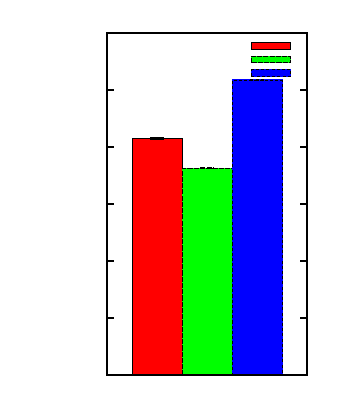
\includegraphics{CumulativeSumSelectL1CM}}%
    \gplfronttext
  \end{picture}%
\endgroup

	\caption{Level 1 Cache Misses}
	\label{fig:CumulativeSumSelectL1CM}
\end{subfigure}


\begin{subfigure}{0.30\textwidth}
	% GNUPLOT: LaTeX picture with Postscript
\begingroup
  \makeatletter
  \providecommand\color[2][]{%
    \GenericError{(gnuplot) \space\space\space\@spaces}{%
      Package color not loaded in conjunction with
      terminal option `colourtext'%
    }{See the gnuplot documentation for explanation.%
    }{Either use 'blacktext' in gnuplot or load the package
      color.sty in LaTeX.}%
    \renewcommand\color[2][]{}%
  }%
  \providecommand\includegraphics[2][]{%
    \GenericError{(gnuplot) \space\space\space\@spaces}{%
      Package graphicx or graphics not loaded%
    }{See the gnuplot documentation for explanation.%
    }{The gnuplot epslatex terminal needs graphicx.sty or graphics.sty.}%
    \renewcommand\includegraphics[2][]{}%
  }%
  \providecommand\rotatebox[2]{#2}%
  \@ifundefined{ifGPcolor}{%
    \newif\ifGPcolor
    \GPcolortrue
  }{}%
  \@ifundefined{ifGPblacktext}{%
    \newif\ifGPblacktext
    \GPblacktexttrue
  }{}%
  % define a \g@addto@macro without @ in the name:
  \let\gplgaddtomacro\g@addto@macro
  % define empty templates for all commands taking text:
  \gdef\gplbacktext{}%
  \gdef\gplfronttext{}%
  \makeatother
  \ifGPblacktext
    % no textcolor at all
    \def\colorrgb#1{}%
    \def\colorgray#1{}%
  \else
    % gray or color?
    \ifGPcolor
      \def\colorrgb#1{\color[rgb]{#1}}%
      \def\colorgray#1{\color[gray]{#1}}%
      \expandafter\def\csname LTw\endcsname{\color{white}}%
      \expandafter\def\csname LTb\endcsname{\color{black}}%
      \expandafter\def\csname LTa\endcsname{\color{black}}%
      \expandafter\def\csname LT0\endcsname{\color[rgb]{1,0,0}}%
      \expandafter\def\csname LT1\endcsname{\color[rgb]{0,1,0}}%
      \expandafter\def\csname LT2\endcsname{\color[rgb]{0,0,1}}%
      \expandafter\def\csname LT3\endcsname{\color[rgb]{1,0,1}}%
      \expandafter\def\csname LT4\endcsname{\color[rgb]{0,1,1}}%
      \expandafter\def\csname LT5\endcsname{\color[rgb]{1,1,0}}%
      \expandafter\def\csname LT6\endcsname{\color[rgb]{0,0,0}}%
      \expandafter\def\csname LT7\endcsname{\color[rgb]{1,0.3,0}}%
      \expandafter\def\csname LT8\endcsname{\color[rgb]{0.5,0.5,0.5}}%
    \else
      % gray
      \def\colorrgb#1{\color{black}}%
      \def\colorgray#1{\color[gray]{#1}}%
      \expandafter\def\csname LTw\endcsname{\color{white}}%
      \expandafter\def\csname LTb\endcsname{\color{black}}%
      \expandafter\def\csname LTa\endcsname{\color{black}}%
      \expandafter\def\csname LT0\endcsname{\color{black}}%
      \expandafter\def\csname LT1\endcsname{\color{black}}%
      \expandafter\def\csname LT2\endcsname{\color{black}}%
      \expandafter\def\csname LT3\endcsname{\color{black}}%
      \expandafter\def\csname LT4\endcsname{\color{black}}%
      \expandafter\def\csname LT5\endcsname{\color{black}}%
      \expandafter\def\csname LT6\endcsname{\color{black}}%
      \expandafter\def\csname LT7\endcsname{\color{black}}%
      \expandafter\def\csname LT8\endcsname{\color{black}}%
    \fi
  \fi
  \setlength{\unitlength}{0.0500bp}%
  \begin{picture}(3024.00,3600.00)%
    \gplgaddtomacro\gplbacktext{%
      \csname LTb\endcsname%
      \put(793,156){\makebox(0,0)[r]{\strut{} 0}}%
      \put(793,788){\makebox(0,0)[r]{\strut{} 50000}}%
      \put(793,1420){\makebox(0,0)[r]{\strut{} 100000}}%
      \put(793,2052){\makebox(0,0)[r]{\strut{} 150000}}%
      \put(793,2684){\makebox(0,0)[r]{\strut{} 200000}}%
      \put(793,3317){\makebox(0,0)[r]{\strut{} 250000}}%
      \put(104,1799){\rotatebox{-270}{\makebox(0,0){\strut{}Cache Misses}}}%
    }%
    \gplgaddtomacro\gplfronttext{%
      \csname LTb\endcsname%
      \put(2180,3315){\makebox(0,0)[r]{\strut{}UnalignedNaive}}%
      \csname LTb\endcsname%
      \put(2180,3185){\makebox(0,0)[r]{\strut{}CumulativeSum}}%
      \csname LTb\endcsname%
      \put(2180,3055){\makebox(0,0)[r]{\strut{}CumSumBranchless}}%
    }%
    \gplbacktext
    \put(0,0){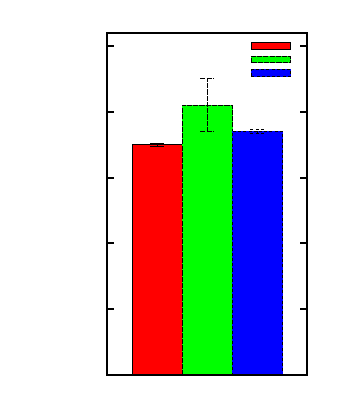
\includegraphics{CumulativeSumSelectL2CM}}%
    \gplfronttext
  \end{picture}%
\endgroup

	\caption{Level 2 Cache Misses}
	\label{fig:CumulativeSumSelectL2CM}
\end{subfigure}
\hfill
\begin{subfigure}{0.30\textwidth}
	% GNUPLOT: LaTeX picture with Postscript
\begingroup
  \makeatletter
  \providecommand\color[2][]{%
    \GenericError{(gnuplot) \space\space\space\@spaces}{%
      Package color not loaded in conjunction with
      terminal option `colourtext'%
    }{See the gnuplot documentation for explanation.%
    }{Either use 'blacktext' in gnuplot or load the package
      color.sty in LaTeX.}%
    \renewcommand\color[2][]{}%
  }%
  \providecommand\includegraphics[2][]{%
    \GenericError{(gnuplot) \space\space\space\@spaces}{%
      Package graphicx or graphics not loaded%
    }{See the gnuplot documentation for explanation.%
    }{The gnuplot epslatex terminal needs graphicx.sty or graphics.sty.}%
    \renewcommand\includegraphics[2][]{}%
  }%
  \providecommand\rotatebox[2]{#2}%
  \@ifundefined{ifGPcolor}{%
    \newif\ifGPcolor
    \GPcolortrue
  }{}%
  \@ifundefined{ifGPblacktext}{%
    \newif\ifGPblacktext
    \GPblacktexttrue
  }{}%
  % define a \g@addto@macro without @ in the name:
  \let\gplgaddtomacro\g@addto@macro
  % define empty templates for all commands taking text:
  \gdef\gplbacktext{}%
  \gdef\gplfronttext{}%
  \makeatother
  \ifGPblacktext
    % no textcolor at all
    \def\colorrgb#1{}%
    \def\colorgray#1{}%
  \else
    % gray or color?
    \ifGPcolor
      \def\colorrgb#1{\color[rgb]{#1}}%
      \def\colorgray#1{\color[gray]{#1}}%
      \expandafter\def\csname LTw\endcsname{\color{white}}%
      \expandafter\def\csname LTb\endcsname{\color{black}}%
      \expandafter\def\csname LTa\endcsname{\color{black}}%
      \expandafter\def\csname LT0\endcsname{\color[rgb]{1,0,0}}%
      \expandafter\def\csname LT1\endcsname{\color[rgb]{0,1,0}}%
      \expandafter\def\csname LT2\endcsname{\color[rgb]{0,0,1}}%
      \expandafter\def\csname LT3\endcsname{\color[rgb]{1,0,1}}%
      \expandafter\def\csname LT4\endcsname{\color[rgb]{0,1,1}}%
      \expandafter\def\csname LT5\endcsname{\color[rgb]{1,1,0}}%
      \expandafter\def\csname LT6\endcsname{\color[rgb]{0,0,0}}%
      \expandafter\def\csname LT7\endcsname{\color[rgb]{1,0.3,0}}%
      \expandafter\def\csname LT8\endcsname{\color[rgb]{0.5,0.5,0.5}}%
    \else
      % gray
      \def\colorrgb#1{\color{black}}%
      \def\colorgray#1{\color[gray]{#1}}%
      \expandafter\def\csname LTw\endcsname{\color{white}}%
      \expandafter\def\csname LTb\endcsname{\color{black}}%
      \expandafter\def\csname LTa\endcsname{\color{black}}%
      \expandafter\def\csname LT0\endcsname{\color{black}}%
      \expandafter\def\csname LT1\endcsname{\color{black}}%
      \expandafter\def\csname LT2\endcsname{\color{black}}%
      \expandafter\def\csname LT3\endcsname{\color{black}}%
      \expandafter\def\csname LT4\endcsname{\color{black}}%
      \expandafter\def\csname LT5\endcsname{\color{black}}%
      \expandafter\def\csname LT6\endcsname{\color{black}}%
      \expandafter\def\csname LT7\endcsname{\color{black}}%
      \expandafter\def\csname LT8\endcsname{\color{black}}%
    \fi
  \fi
  \setlength{\unitlength}{0.0500bp}%
  \begin{picture}(3024.00,3600.00)%
    \gplgaddtomacro\gplbacktext{%
      \csname LTb\endcsname%
      \put(793,156){\makebox(0,0)[r]{\strut{} 0}}%
      \put(793,626){\makebox(0,0)[r]{\strut{} 50000}}%
      \put(793,1095){\makebox(0,0)[r]{\strut{} 100000}}%
      \put(793,1565){\makebox(0,0)[r]{\strut{} 150000}}%
      \put(793,2034){\makebox(0,0)[r]{\strut{} 200000}}%
      \put(793,2504){\makebox(0,0)[r]{\strut{} 250000}}%
      \put(793,2973){\makebox(0,0)[r]{\strut{} 300000}}%
      \put(793,3443){\makebox(0,0)[r]{\strut{} 350000}}%
      \put(104,1799){\rotatebox{-270}{\makebox(0,0){\strut{}Cache Hits}}}%
    }%
    \gplgaddtomacro\gplfronttext{%
      \csname LTb\endcsname%
      \put(2180,3315){\makebox(0,0)[r]{\strut{}UnalignedNaive}}%
      \csname LTb\endcsname%
      \put(2180,3185){\makebox(0,0)[r]{\strut{}CumulativeSum}}%
      \csname LTb\endcsname%
      \put(2180,3055){\makebox(0,0)[r]{\strut{}CumSumBranchless}}%
    }%
    \gplbacktext
    \put(0,0){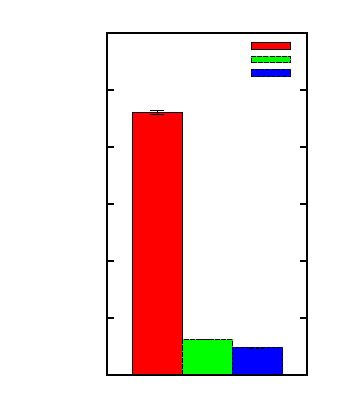
\includegraphics{CumulativeSumSelectL2CHits}}%
    \gplfronttext
  \end{picture}%
\endgroup

	\caption{Level 2 Cache Hits}
	\label{fig:CumulativeSumSelectL2CHits}
\end{subfigure}
\hfill
%\begin{subfigure}{0.30\textwidth}
%	% GNUPLOT: LaTeX picture with Postscript
\begingroup
  \makeatletter
  \providecommand\color[2][]{%
    \GenericError{(gnuplot) \space\space\space\@spaces}{%
      Package color not loaded in conjunction with
      terminal option `colourtext'%
    }{See the gnuplot documentation for explanation.%
    }{Either use 'blacktext' in gnuplot or load the package
      color.sty in LaTeX.}%
    \renewcommand\color[2][]{}%
  }%
  \providecommand\includegraphics[2][]{%
    \GenericError{(gnuplot) \space\space\space\@spaces}{%
      Package graphicx or graphics not loaded%
    }{See the gnuplot documentation for explanation.%
    }{The gnuplot epslatex terminal needs graphicx.sty or graphics.sty.}%
    \renewcommand\includegraphics[2][]{}%
  }%
  \providecommand\rotatebox[2]{#2}%
  \@ifundefined{ifGPcolor}{%
    \newif\ifGPcolor
    \GPcolortrue
  }{}%
  \@ifundefined{ifGPblacktext}{%
    \newif\ifGPblacktext
    \GPblacktexttrue
  }{}%
  % define a \g@addto@macro without @ in the name:
  \let\gplgaddtomacro\g@addto@macro
  % define empty templates for all commands taking text:
  \gdef\gplbacktext{}%
  \gdef\gplfronttext{}%
  \makeatother
  \ifGPblacktext
    % no textcolor at all
    \def\colorrgb#1{}%
    \def\colorgray#1{}%
  \else
    % gray or color?
    \ifGPcolor
      \def\colorrgb#1{\color[rgb]{#1}}%
      \def\colorgray#1{\color[gray]{#1}}%
      \expandafter\def\csname LTw\endcsname{\color{white}}%
      \expandafter\def\csname LTb\endcsname{\color{black}}%
      \expandafter\def\csname LTa\endcsname{\color{black}}%
      \expandafter\def\csname LT0\endcsname{\color[rgb]{1,0,0}}%
      \expandafter\def\csname LT1\endcsname{\color[rgb]{0,1,0}}%
      \expandafter\def\csname LT2\endcsname{\color[rgb]{0,0,1}}%
      \expandafter\def\csname LT3\endcsname{\color[rgb]{1,0,1}}%
      \expandafter\def\csname LT4\endcsname{\color[rgb]{0,1,1}}%
      \expandafter\def\csname LT5\endcsname{\color[rgb]{1,1,0}}%
      \expandafter\def\csname LT6\endcsname{\color[rgb]{0,0,0}}%
      \expandafter\def\csname LT7\endcsname{\color[rgb]{1,0.3,0}}%
      \expandafter\def\csname LT8\endcsname{\color[rgb]{0.5,0.5,0.5}}%
    \else
      % gray
      \def\colorrgb#1{\color{black}}%
      \def\colorgray#1{\color[gray]{#1}}%
      \expandafter\def\csname LTw\endcsname{\color{white}}%
      \expandafter\def\csname LTb\endcsname{\color{black}}%
      \expandafter\def\csname LTa\endcsname{\color{black}}%
      \expandafter\def\csname LT0\endcsname{\color{black}}%
      \expandafter\def\csname LT1\endcsname{\color{black}}%
      \expandafter\def\csname LT2\endcsname{\color{black}}%
      \expandafter\def\csname LT3\endcsname{\color{black}}%
      \expandafter\def\csname LT4\endcsname{\color{black}}%
      \expandafter\def\csname LT5\endcsname{\color{black}}%
      \expandafter\def\csname LT6\endcsname{\color{black}}%
      \expandafter\def\csname LT7\endcsname{\color{black}}%
      \expandafter\def\csname LT8\endcsname{\color{black}}%
    \fi
  \fi
  \setlength{\unitlength}{0.0500bp}%
  \begin{picture}(3024.00,3600.00)%
    \gplgaddtomacro\gplbacktext{%
      \csname LTb\endcsname%
      \put(559,156){\makebox(0,0)[r]{\strut{} 0}}%
      \put(559,567){\makebox(0,0)[r]{\strut{} 0.2}}%
      \put(559,978){\makebox(0,0)[r]{\strut{} 0.4}}%
      \put(559,1389){\makebox(0,0)[r]{\strut{} 0.6}}%
      \put(559,1800){\makebox(0,0)[r]{\strut{} 0.8}}%
      \put(559,2210){\makebox(0,0)[r]{\strut{} 1}}%
      \put(559,2621){\makebox(0,0)[r]{\strut{} 1.2}}%
      \put(559,3032){\makebox(0,0)[r]{\strut{} 1.4}}%
      \put(559,3443){\makebox(0,0)[r]{\strut{} 1.6}}%
      \put(104,1799){\rotatebox{-270}{\makebox(0,0){\strut{}Cache Miss Rate}}}%
    }%
    \gplgaddtomacro\gplfronttext{%
      \csname LTb\endcsname%
      \put(2180,3315){\makebox(0,0)[r]{\strut{}UnalignedNaive}}%
      \csname LTb\endcsname%
      \put(2180,3185){\makebox(0,0)[r]{\strut{}CumulativeSum}}%
      \csname LTb\endcsname%
      \put(2180,3055){\makebox(0,0)[r]{\strut{}CmSumBranchless}}%
    }%
    \gplbacktext
    \put(0,0){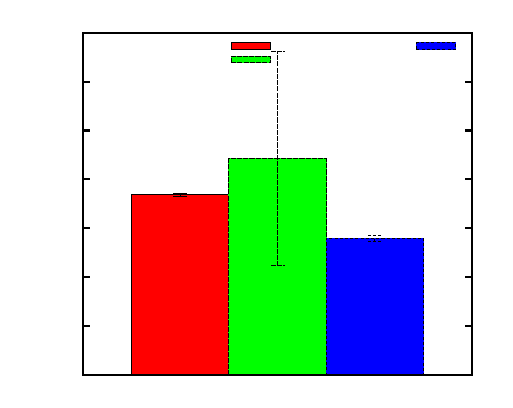
\includegraphics{CumulativeSumSelectL2CMRate}}%
    \gplfronttext
  \end{picture}%
\endgroup

%	\caption{Level 2 Cache Miss Rate}
%	\label{fig:CumulativeSumSelectL2CMRate}
%\end{subfigure}
%\hfill
\begin{subfigure}{0.30\textwidth}
	% GNUPLOT: LaTeX picture with Postscript
\begingroup
  \makeatletter
  \providecommand\color[2][]{%
    \GenericError{(gnuplot) \space\space\space\@spaces}{%
      Package color not loaded in conjunction with
      terminal option `colourtext'%
    }{See the gnuplot documentation for explanation.%
    }{Either use 'blacktext' in gnuplot or load the package
      color.sty in LaTeX.}%
    \renewcommand\color[2][]{}%
  }%
  \providecommand\includegraphics[2][]{%
    \GenericError{(gnuplot) \space\space\space\@spaces}{%
      Package graphicx or graphics not loaded%
    }{See the gnuplot documentation for explanation.%
    }{The gnuplot epslatex terminal needs graphicx.sty or graphics.sty.}%
    \renewcommand\includegraphics[2][]{}%
  }%
  \providecommand\rotatebox[2]{#2}%
  \@ifundefined{ifGPcolor}{%
    \newif\ifGPcolor
    \GPcolortrue
  }{}%
  \@ifundefined{ifGPblacktext}{%
    \newif\ifGPblacktext
    \GPblacktexttrue
  }{}%
  % define a \g@addto@macro without @ in the name:
  \let\gplgaddtomacro\g@addto@macro
  % define empty templates for all commands taking text:
  \gdef\gplbacktext{}%
  \gdef\gplfronttext{}%
  \makeatother
  \ifGPblacktext
    % no textcolor at all
    \def\colorrgb#1{}%
    \def\colorgray#1{}%
  \else
    % gray or color?
    \ifGPcolor
      \def\colorrgb#1{\color[rgb]{#1}}%
      \def\colorgray#1{\color[gray]{#1}}%
      \expandafter\def\csname LTw\endcsname{\color{white}}%
      \expandafter\def\csname LTb\endcsname{\color{black}}%
      \expandafter\def\csname LTa\endcsname{\color{black}}%
      \expandafter\def\csname LT0\endcsname{\color[rgb]{1,0,0}}%
      \expandafter\def\csname LT1\endcsname{\color[rgb]{0,1,0}}%
      \expandafter\def\csname LT2\endcsname{\color[rgb]{0,0,1}}%
      \expandafter\def\csname LT3\endcsname{\color[rgb]{1,0,1}}%
      \expandafter\def\csname LT4\endcsname{\color[rgb]{0,1,1}}%
      \expandafter\def\csname LT5\endcsname{\color[rgb]{1,1,0}}%
      \expandafter\def\csname LT6\endcsname{\color[rgb]{0,0,0}}%
      \expandafter\def\csname LT7\endcsname{\color[rgb]{1,0.3,0}}%
      \expandafter\def\csname LT8\endcsname{\color[rgb]{0.5,0.5,0.5}}%
    \else
      % gray
      \def\colorrgb#1{\color{black}}%
      \def\colorgray#1{\color[gray]{#1}}%
      \expandafter\def\csname LTw\endcsname{\color{white}}%
      \expandafter\def\csname LTb\endcsname{\color{black}}%
      \expandafter\def\csname LTa\endcsname{\color{black}}%
      \expandafter\def\csname LT0\endcsname{\color{black}}%
      \expandafter\def\csname LT1\endcsname{\color{black}}%
      \expandafter\def\csname LT2\endcsname{\color{black}}%
      \expandafter\def\csname LT3\endcsname{\color{black}}%
      \expandafter\def\csname LT4\endcsname{\color{black}}%
      \expandafter\def\csname LT5\endcsname{\color{black}}%
      \expandafter\def\csname LT6\endcsname{\color{black}}%
      \expandafter\def\csname LT7\endcsname{\color{black}}%
      \expandafter\def\csname LT8\endcsname{\color{black}}%
    \fi
  \fi
  \setlength{\unitlength}{0.0500bp}%
  \begin{picture}(3024.00,3600.00)%
    \gplgaddtomacro\gplbacktext{%
      \csname LTb\endcsname%
      \put(793,156){\makebox(0,0)[r]{\strut{} 0}}%
      \put(793,841){\makebox(0,0)[r]{\strut{} 50000}}%
      \put(793,1526){\makebox(0,0)[r]{\strut{} 100000}}%
      \put(793,2210){\makebox(0,0)[r]{\strut{} 150000}}%
      \put(793,2895){\makebox(0,0)[r]{\strut{} 200000}}%
      \put(104,1799){\rotatebox{-270}{\makebox(0,0){\strut{}Cache Misses}}}%
    }%
    \gplgaddtomacro\gplfronttext{%
      \csname LTb\endcsname%
      \put(2180,3315){\makebox(0,0)[r]{\strut{}UnalignedNaive}}%
      \csname LTb\endcsname%
      \put(2180,3185){\makebox(0,0)[r]{\strut{}CumulativeSum}}%
      \csname LTb\endcsname%
      \put(2180,3055){\makebox(0,0)[r]{\strut{}CumSumBranchless}}%
    }%
    \gplbacktext
    \put(0,0){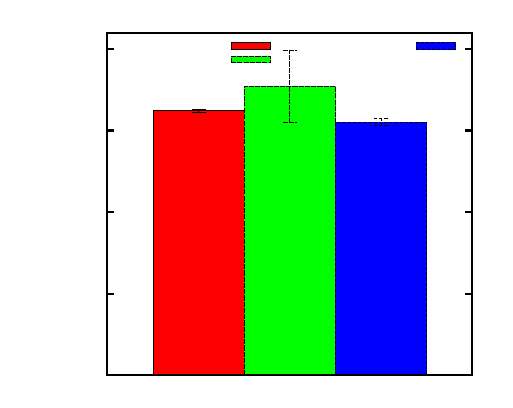
\includegraphics{CumulativeSumSelectL3CM}}%
    \gplfronttext
  \end{picture}%
\endgroup

	\caption{Level 3 Cache Misses Rate}
	\label{fig:CumulativeSumSelectL3CM}
\end{subfigure}

\caption{Measurements on Select Queries on the UnalignedNaive and CumulativeSum and CumulativeSumBranchless Wavelet Trees. Part 1.}
\label{fig:CumulativeSumSelect}
\end{figure}





\restoregeometry













